% ============================================================================
% AI 漫剧制作平台实训报告（LaTeX 版）
% 编译方式（需要 ctex 宏包与 xelatex）：
%   xelatex AI漫剧制作平台实训报告.tex
% 表格使用 longtable 支持跨页，代码使用 listings 标注语言。
% ============================================================================
\documentclass[12pt]{ctexrep}
\usepackage[a4paper,left=2.6cm,right=2.6cm,top=2.8cm,bottom=2.8cm]{geometry}
\usepackage{booktabs}
\usepackage{longtable}
\usepackage{array}
\usepackage{listings}
\usepackage{xcolor}
\usepackage{graphicx}
\usepackage{hyperref}
\usepackage{setspace}
\hypersetup{colorlinks=true,linkcolor=blue,urlcolor=blue}

% 等宽字体：verbatim/listings 中的中文与框线字符（┌─┐│）需要支持 CJK+Box Drawing 的字体
\usepackage{fontspec}
\setmonofont{Menlo}[Scale=0.85]
\xeCJKsetcharclass{"2500}{"257F}{1}   % Box Drawing 字符归入 CJK 类，由中文字体渲染

% ---- 代码样式 ----
\lstset{
  basicstyle=\ttfamily\footnotesize,
  keywordstyle=\color{blue}\bfseries,
  commentstyle=\color{gray},
  stringstyle=\color{red!70!black},
  numbers=left, numberstyle=\tiny\color{gray},
  frame=single, rulecolor=\color{gray!50},
  breaklines=true, showstringspaces=false,
  language=Python
}

\setcounter{tocdepth}{2}
\begin{document}

% ============================================================================
\title{\bfseries AI 漫剧制作平台实训报告}
\author{湖南师范大学 \quad 信息与计算科学专业\\
学号：202330124036 \quad 姓名：潘磊}
\date{\today}
\maketitle

\begin{center}
\begin{minipage}{0.9\textwidth}
\textbf{项目定位：}面向短剧制作团队的多镜头 AI 漫剧（视频短剧）全流程生产平台\\
\textbf{技术路线：}Python + FastAPI + Vue 3 + FFmpeg + 国产大模型生态
\end{minipage}
\end{center}

\tableofcontents

% ============================================================================
\chapter{项目背景与意义}
\section{项目背景}
\subsection{AIGC 与多模态大模型的发展趋势}

2023 年以来，以 ChatGPT 为代表的大语言模型（LLM）掀起了 AIGC（AI 生成内容）浪潮，随后多模态大模型快速演进：文本生成（DeepSeek、通义千问、Kimi）、文生图（可图 Kolors、混元）、文生视频（可灵 Kling、即梦）以及语音合成（CosyVoice、火山引擎）在短短两年内完成了从实验室到规模商用的跨越。

在这一背景下，内容生产行业的范式正在被重构：传统短剧制作需要编剧、导演、画师、配音、剪辑等多人协作，单集成本高、周期长。而 AIGC 工具链的出现，使得「一个人 + 一套 AI 工作流」即可产出接近成片的漫剧内容，短剧行业迎来生产方式的重大变革。

\subsection{市场同类产品现状分析}

\begin{longtable}{p{3cm}p{3.4cm}p{4.4cm}p{5.2cm}}
\caption{同类产品对比分析}\label{tab:competitors}\\
\toprule
竞品 & 定位 & 优势 & 不足\\
\midrule
\endfirsthead
\toprule
竞品 & 定位 & 优势 & 不足\\
\midrule
\endhead
可灵 AI（快手） & AI 视频生成 & 视频生成质量高、运镜自然 & 单次生成片段短、无剧本到成片的完整编排\\
即梦 AI（字节） & AI 图像/视频创作 & 图像质量好、社区活跃 & 面向单图/单段视频，缺乏产品化流程\\
剪映（CapCut） & 视频剪辑 & 剪辑强大、模板丰富 & 无剧本与分镜生成，配音需人工逐段制作\\
各类 AI 漫剧工具 & 图片转动态漫剧 & 一键生成短剧 & 缺角色一致性、字幕烧录与镜头语言设计\\
\bottomrule
\end{longtable}

\subsection{现有方案的不足或痛点}

\begin{enumerate}
\item \textbf{流程割裂}：剧本、分镜、图片、配音、视频各环节分散在不同工具中，创作者需反复搬运数据。
\item \textbf{新人门槛高}：完整漫剧生产涉及大量专业术语（镜头类型、机位、情绪强度、声线组合），自由创作模式对新人不友好。
\item \textbf{质量不可控}：无模板约束时，AI 生成内容天马行空，难以符合短剧节奏感与爽点结构。
\item \textbf{环境依赖重}：多数方案强依赖付费 API，缺少本地可演示、可降级的轻量实现。
\end{enumerate}

\section{项目意义}
\subsection{解决的实际问题}

本项目以\textbf{模板驱动 + 全流程编排}为核心思路，解决“从一部小说到一段可发布的漫剧视频”这一完整问题：创作者只需选择模板、填写少量必填变量，系统即可自动完成剧本合成、分镜拆解、图片批量生成、配音合成与视频合成，将原来数小时的手工流程压缩到几分钟。

\subsection{对目标用户的价值}

\begin{itemize}
\item \textbf{短剧制作团队}：通过模板批量生产降低单集成本，情绪曲线与分镜结构预设保证成片质量下限。
\item \textbf{内容运营人员}：模板变量（主角名、金句、场景）可快速试错不同人设组合，用于 A/B 测试选题。
\end{itemize}

\subsection{技术价值与学习价值}

技术上，项目覆盖了 LLM Prompt 工程、多模态 API 封装、异步任务编排（线程池 + 信号量并发）、视频处理（FFmpeg 滤镜链、Ken Burns 效果、字幕烧录）、RESTful 接口设计、ORM 建模与前端工程化等内容；学习上，完整实践了“需求分析 → 架构设计 → 模块实现 → 测试验证”的软件工程闭环。

% ============================================================================
\chapter{需求分析}
\section{用户角色}

\begin{table}[htbp]
\centering
\begin{tabular}{p{3.2cm}p{6cm}p{5.5cm}}
\toprule
角色 & 说明 & 主要权限\\
\midrule
普通用户（创作者） & 使用模板生成漫剧、管理自己的项目/角色/场景/素材 & 创建与编辑自己的项目与素材\\
管理员 & 平台运营与内容维护 & 全部数据访问、模板维护（以默认 admin 账号体现）\\
\bottomrule
\end{tabular}
\caption{用户角色定义}\label{tab:roles}
\end{table}

\section{功能性需求（M1-M4）}

项目按四大功能模块划分，覆盖实训评分表中的全部评分点（AI 剧本生成 10 分、分镜脚本 10 分、分镜图片生成 20 分、分镜图片转视频 20 分、短视频合成剪辑 20 分、配音 10 分、其它创新 10 分）。

\subsection{M1：AI 剧本生成与分镜脚本模块}

\begin{longtable}{p{1.6cm}p{4cm}p{9.4cm}}
\caption{M1 功能点清单}\label{tab:m1}\\
\toprule
编号 & 功能点 & 描述\\
\midrule
\endfirsthead
\toprule
编号 & 功能点 & 描述\\
\midrule
\endhead
M1-1 & 小说导入与剧本生成 & 输入小说/剧情梗概，调用 LLM 生成剧本\\
M1-2 & 分镜脚本拆解 & 拆解为多镜头结构（镜头类型、机位、台词、情绪）\\
M1-3 & 模板变量渲染 & 将模板脚本中的 \$\{变量\} 替换为用户填写值\\
M1-4 & Mock 降级 & 未配置 LLM API Key 时降级为内置 Mock 分镜\\
\bottomrule
\end{longtable}

\subsection{M2：分镜图片生成模块}

\begin{longtable}{p{1.6cm}p{4cm}p{9.4cm}}
\caption{M2 功能点清单}\label{tab:m2}\\
\toprule
编号 & 功能点 & 描述\\
\midrule
\endfirsthead
\toprule
编号 & 功能点 & 描述\\
\midrule
\endhead
M2-1 & 单镜图片生成任务 & 提交单张分镜图生成任务并轮询状态\\
M2-2 & 批量图片调度 & 一个分镜脚本并发调度多镜生成（线程池 + 信号量限流）\\
M2-3 & 生成进度跟踪 & 批量粒度统计完成数/总数与进度百分比\\
M2-4 & 失败状态回传 & 单镜失败记录错误信息，不影响整批任务\\
\bottomrule
\end{longtable}

\subsection{M3：配音合成模块}

\begin{longtable}{p{1.6cm}p{4cm}p{9.4cm}}
\caption{M3 功能点清单}\label{tab:m3}\\
\toprule
编号 & 功能点 & 描述\\
\midrule
\endfirsthead
\toprule
编号 & 功能点 & 描述\\
\midrule
\endhead
M3-1 & 音色列表查询 & 提供多音色（男/女/童声等）供选择\\
M3-2 & 台词转语音 & 输入台词文本与情绪生成配音音频\\
M3-3 & 情绪驱动时长 & 不同情绪（平静/愤怒/悲伤）影响语速与时长\\
M3-4 & 引擎可插拔 & 抽象 TTS 接口，Mock / Edge-TTS 可切换\\
\bottomrule
\end{longtable}

\subsection{M4：视频合成与剪辑模块}

\begin{longtable}{p{1.6cm}p{4cm}p{9.4cm}}
\caption{M4 功能点清单}\label{tab:m4}\\
\toprule
编号 & 功能点 & 描述\\
\midrule
\endfirsthead
\toprule
编号 & 功能点 & 描述\\
\midrule
\endhead
M4-1 & 图片+音频+字幕合成 & 将单镜图片与配音合成视频片段\\
M4-2 & 时长严格对齐 & 视频时长与音频时长偏差 < 0.1s\\
M4-3 & Ken Burns 运镜 & 对静态图施加推/拉镜头动态效果\\
M4-4 & 字幕烧录 & 台词自动烧录为底部字幕（换行、居中、描边）\\
M4-5 & 输出校验 & 输出 H.264 + AAC 标准 mp4，可在线播放\\
\bottomrule
\end{longtable}

\subsection{用例图（Use Case Diagram）}

系统核心用例关系如图 \ref{fig:usecase} 所示：普通用户与管理员围绕模板、生成任务与素材展开交互；剧本生成、分镜生成、图片生成、配音生成、视频合成五个核心用例由系统统一编排，"一键生成"用例内部依次触发图片、配音与视频合成三个子用例。

\begin{figure}[htbp]
\centering
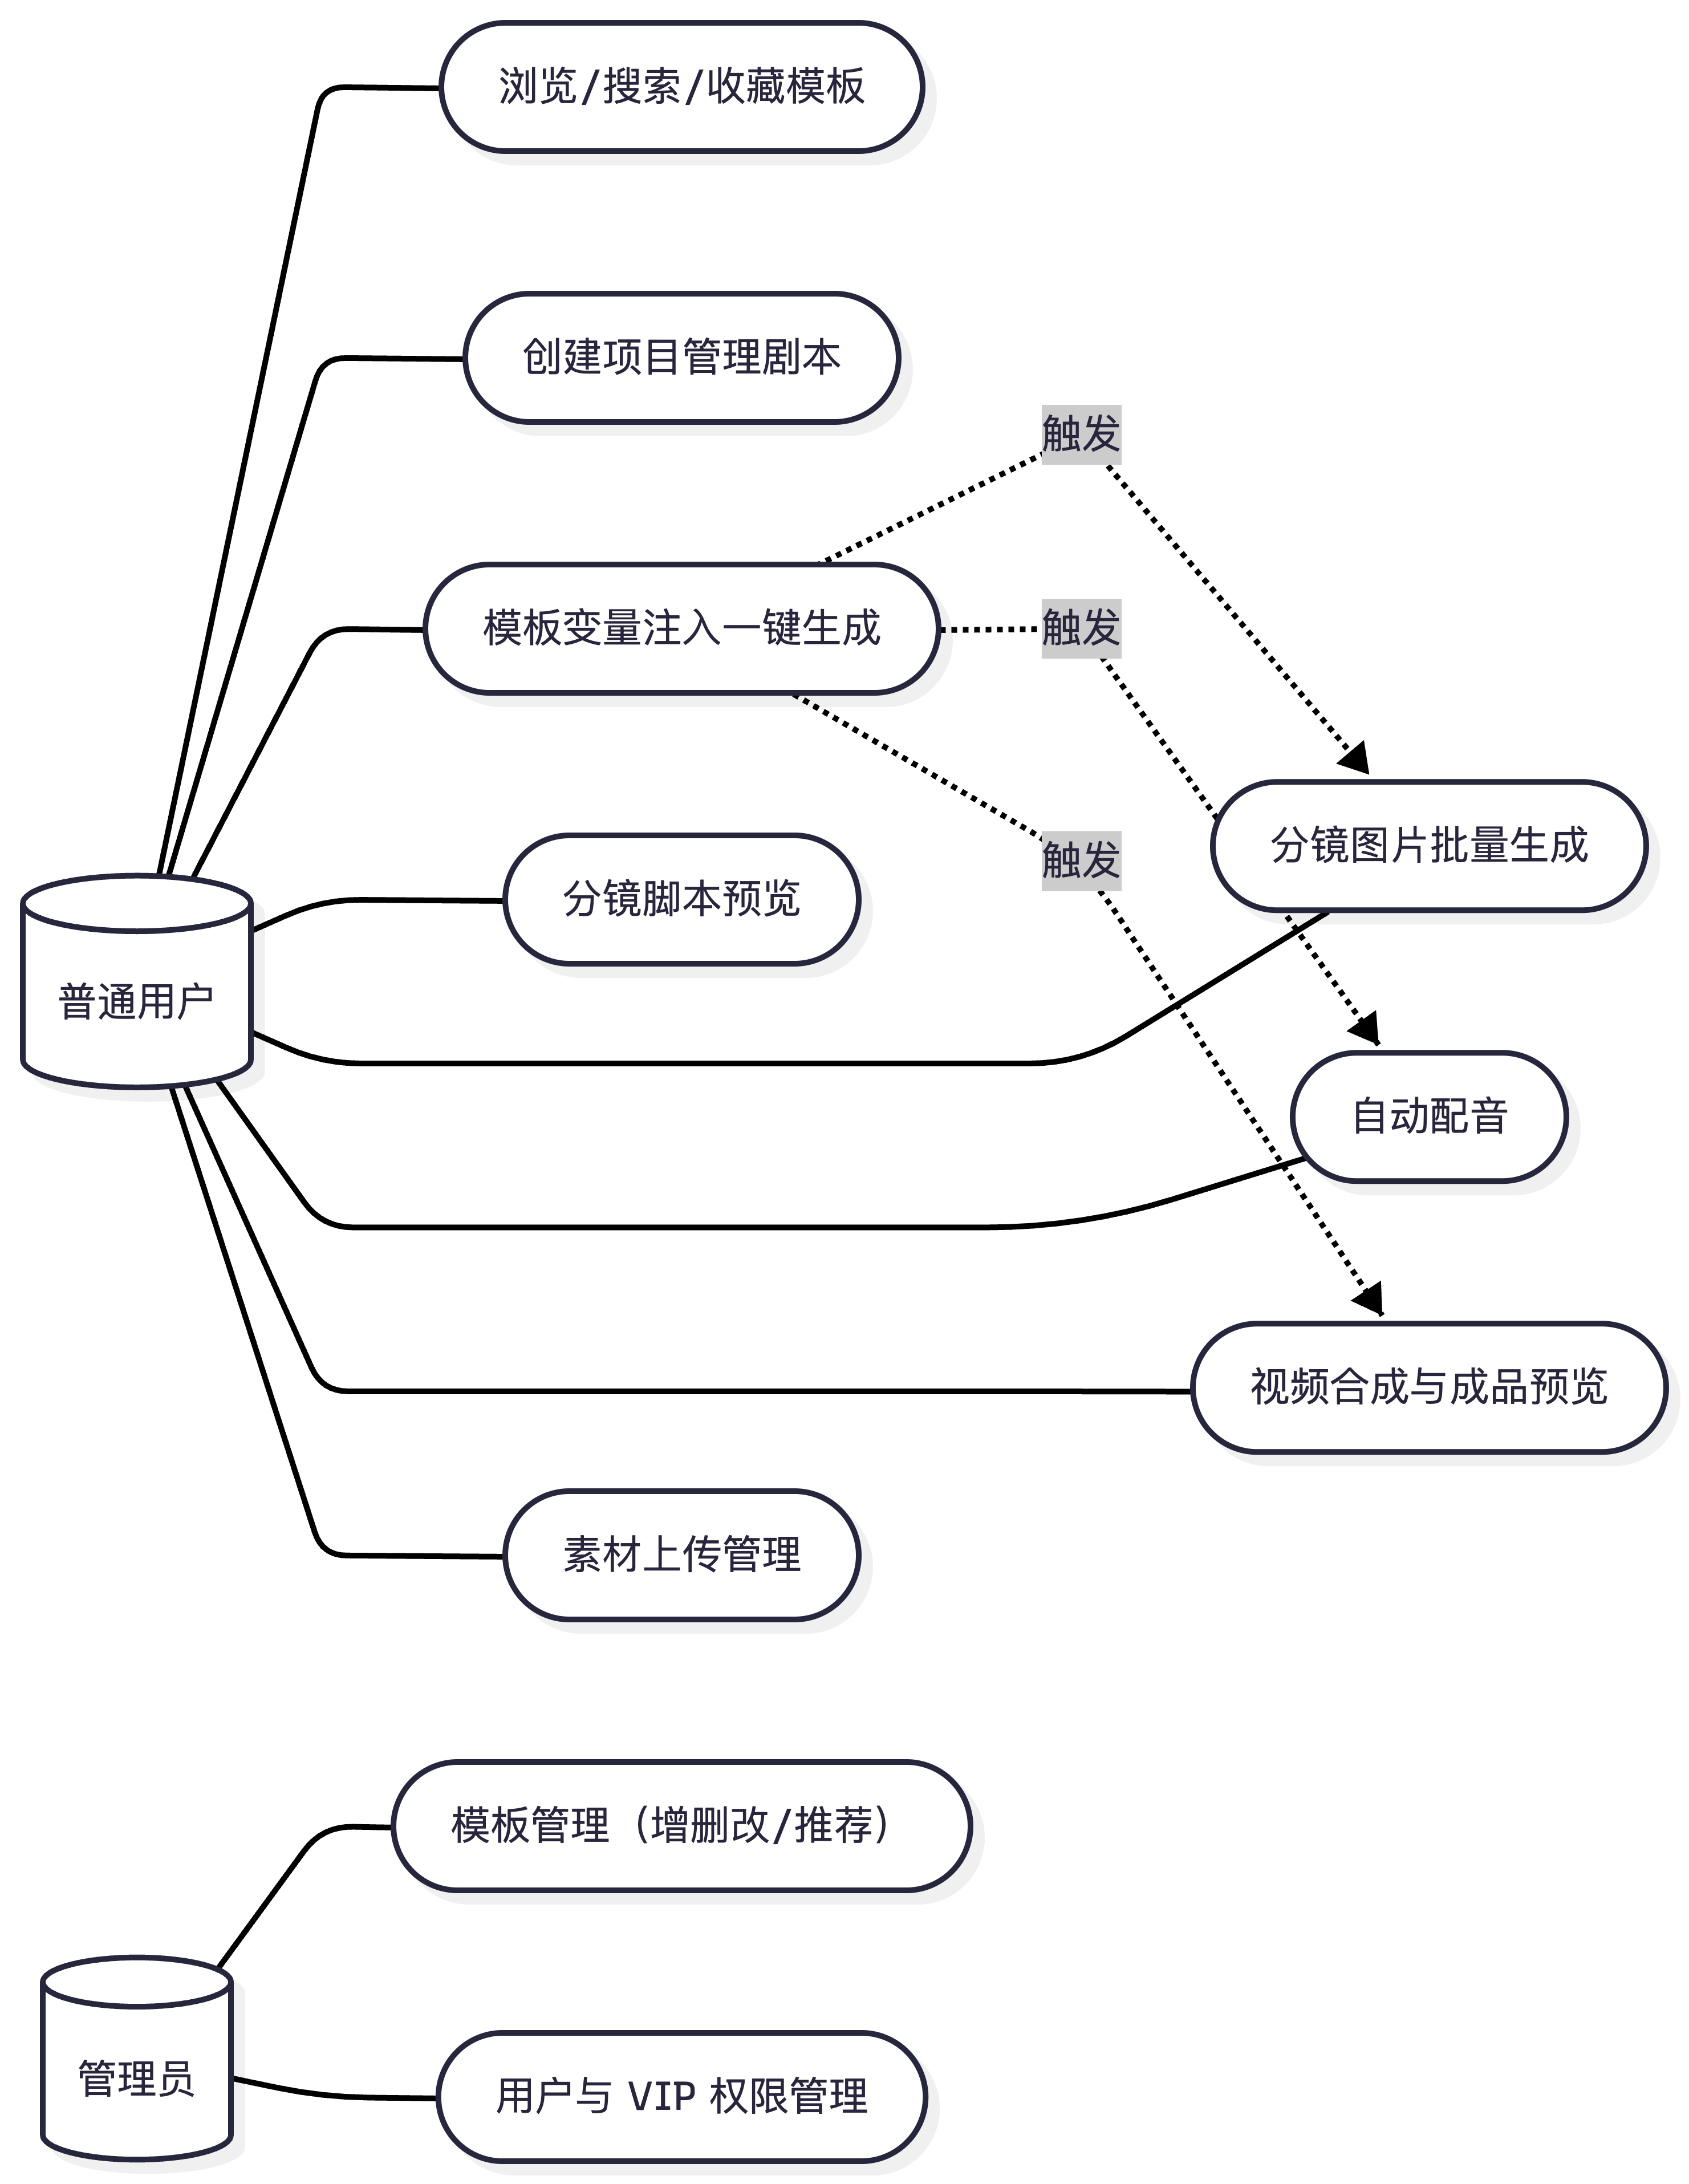
\includegraphics[width=0.62\textwidth]{assets/usecase.png}
\caption{系统用例图}\label{fig:usecase}
\end{figure}

\section{非功能性需求}

\begin{longtable}{p{2.4cm}p{12.6cm}}
\caption{非功能性需求}\label{tab:nonfunc}\\
\toprule
类别 & 需求说明\\
\midrule
\endfirsthead
\toprule
类别 & 需求说明\\
\midrule
\endhead
性能 & 单镜图片生成与配音合成接口响应 < 2s（Mock 模式）；批量 6 镜并发生成 30s 内完成\\
可用性 & 界面友好，新手 3 步内完成一次模板生成；错误信息以中文提示\\
安全性 & JWT Token 认证（生产模式）；密码 bcrypt 加密存储；上传文件大小限制 50MB\\
可扩展性 & TTS、图像生成以抽象接口实现，可无缝切换真实 AI 引擎\\
健壮性 & 无 LLM Key / 无真实 TTS / 精简 FFmpeg 环境均能降级运行并给出明确错误\\
\bottomrule
\end{longtable}

\section{需求优先级}

\begin{longtable}{p{2.4cm}p{6cm}p{6.6cm}}
\caption{需求优先级划分}\label{tab:priority}\\
\toprule
优先级 & 需求 & 说明\\
\midrule
\endfirsthead
\toprule
优先级 & 需求 & 说明\\
\midrule
\endhead
P0（必须） & M1 剧本与分镜、M2 图片、M3 配音、M4 视频合成 & 构成完整业务闭环，缺一不可\\
P1（重要） & 模板驱动批量生产、时长严格对齐、进度可视化 & 决定成片质量与用户体验\\
P2（可选） & 角色一致性、情绪曲线预设、收藏模板、AI 变量补全 & 锦上添花的增强功能\\
\bottomrule
\end{longtable}

% ============================================================================
\chapter{系统架构设计}
\section{架构概述}

系统采用分层架构，自上而下分为前端层、后端层、AI 服务层与数据层四层，整体架构如图 \ref{fig:arch} 所示：

\begin{figure}[htbp]
\centering
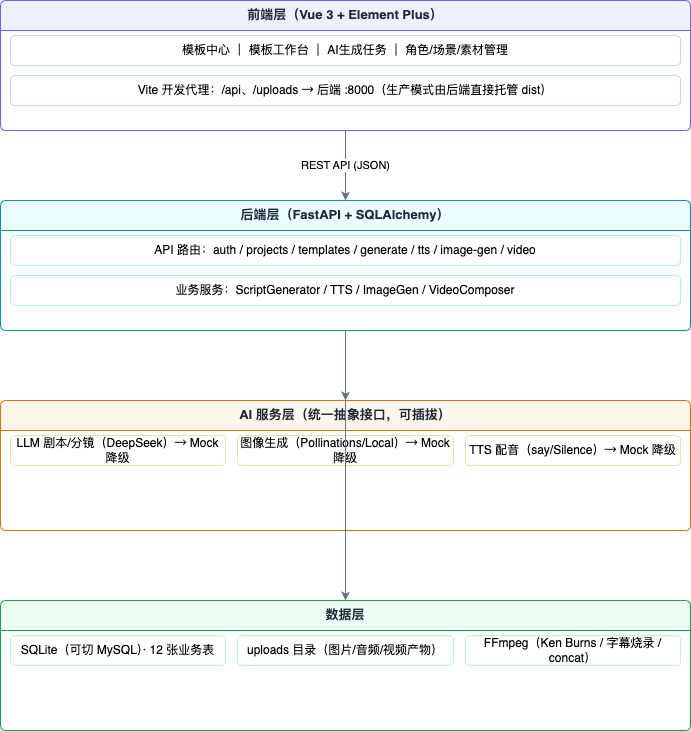
\includegraphics[width=0.8\textwidth]{assets/architecture.png}
\caption{系统整体架构图}\label{fig:arch}
\end{figure}

\textbf{各层职责}：前端层负责用户交互与状态管理，通过 Axios 调用后端 API，开发环境由 Vite 代理转发请求；后端层提供 RESTful API 并承载业务逻辑与任务编排，生成任务采用「提交 → 后台线程执行 → 前端轮询」的异步模型；AI 服务层通过 \texttt{BaseTTSService}、\texttt{BaseImageGenerator} 等抽象接口屏蔽具体 AI 厂商差异，未配置 Key 时自动降级 Mock；数据层以 SQLAlchemy ORM 管理 12 张业务表，媒体产物落盘到 uploads 目录并由静态服务对外提供访问。

\section{模块设计}

四大模块与前后端的对应关系如图 \ref{fig:modules} 所示：

\begin{figure}[htbp]
\centering
\begin{minipage}{0.92\textwidth}
\begin{verbatim}
┌─ 前端页面 ─────────────────────────────────────────────────┐
│ 模板中心 → 模板工作台 → AI生成 → 生成任务进度 → 成品预览    │
└────────────────────────────────────────────────────────────┘
                           │ REST API
┌─ 后端模块 ─────────────────────────────────────────────────┐
│  M1 script_generator 路由+服务（剧本/分镜生成）              │
│  M2 image_generator 路由 + image_gen/batch（图片调度）       │
│  M3 tts 路由 + tts/mock（配音合成）                          │
│  M4 video 路由 + video_composer（视频合成）                  │
│  generate 路由（模板变量注入 + 生成任务状态机）              │
└────────────────────────────────────────────────────────────┘
\end{verbatim}
\end{minipage}
\caption{模块划分与集成关系图}\label{fig:modules}
\end{figure}

模块间以\textbf{生成任务（GenerationTask）}为中枢解耦：M1 产出分镜数据 → M2 按分镜批量生成图片 → M3 生成配音 → M4 合成视频，各模块仅通过数据库记录与文件路径传递产物，互不直接依赖。

\section{数据流向}

\textbf{核心业务流程数据流向}（模板驱动生成，如图 \ref{fig:flow}）：用户输入模板变量 → \texttt{generate} 路由创建 GenerationTask（pending）→ 后台线程注入变量渲染模板脚本（M1）→ 按模板固定分镜生成 GeneratedShot（M1）→ 逐镜提交图片生成任务，BatchImageService 并发调度（M2）→ 逐镜生成配音音频（M3）→ VideoComposer 逐镜合成视频片段（M4）→ 任务置为 done，前端轮询到 100\% 展示成品。

\begin{figure}[htbp]
\centering
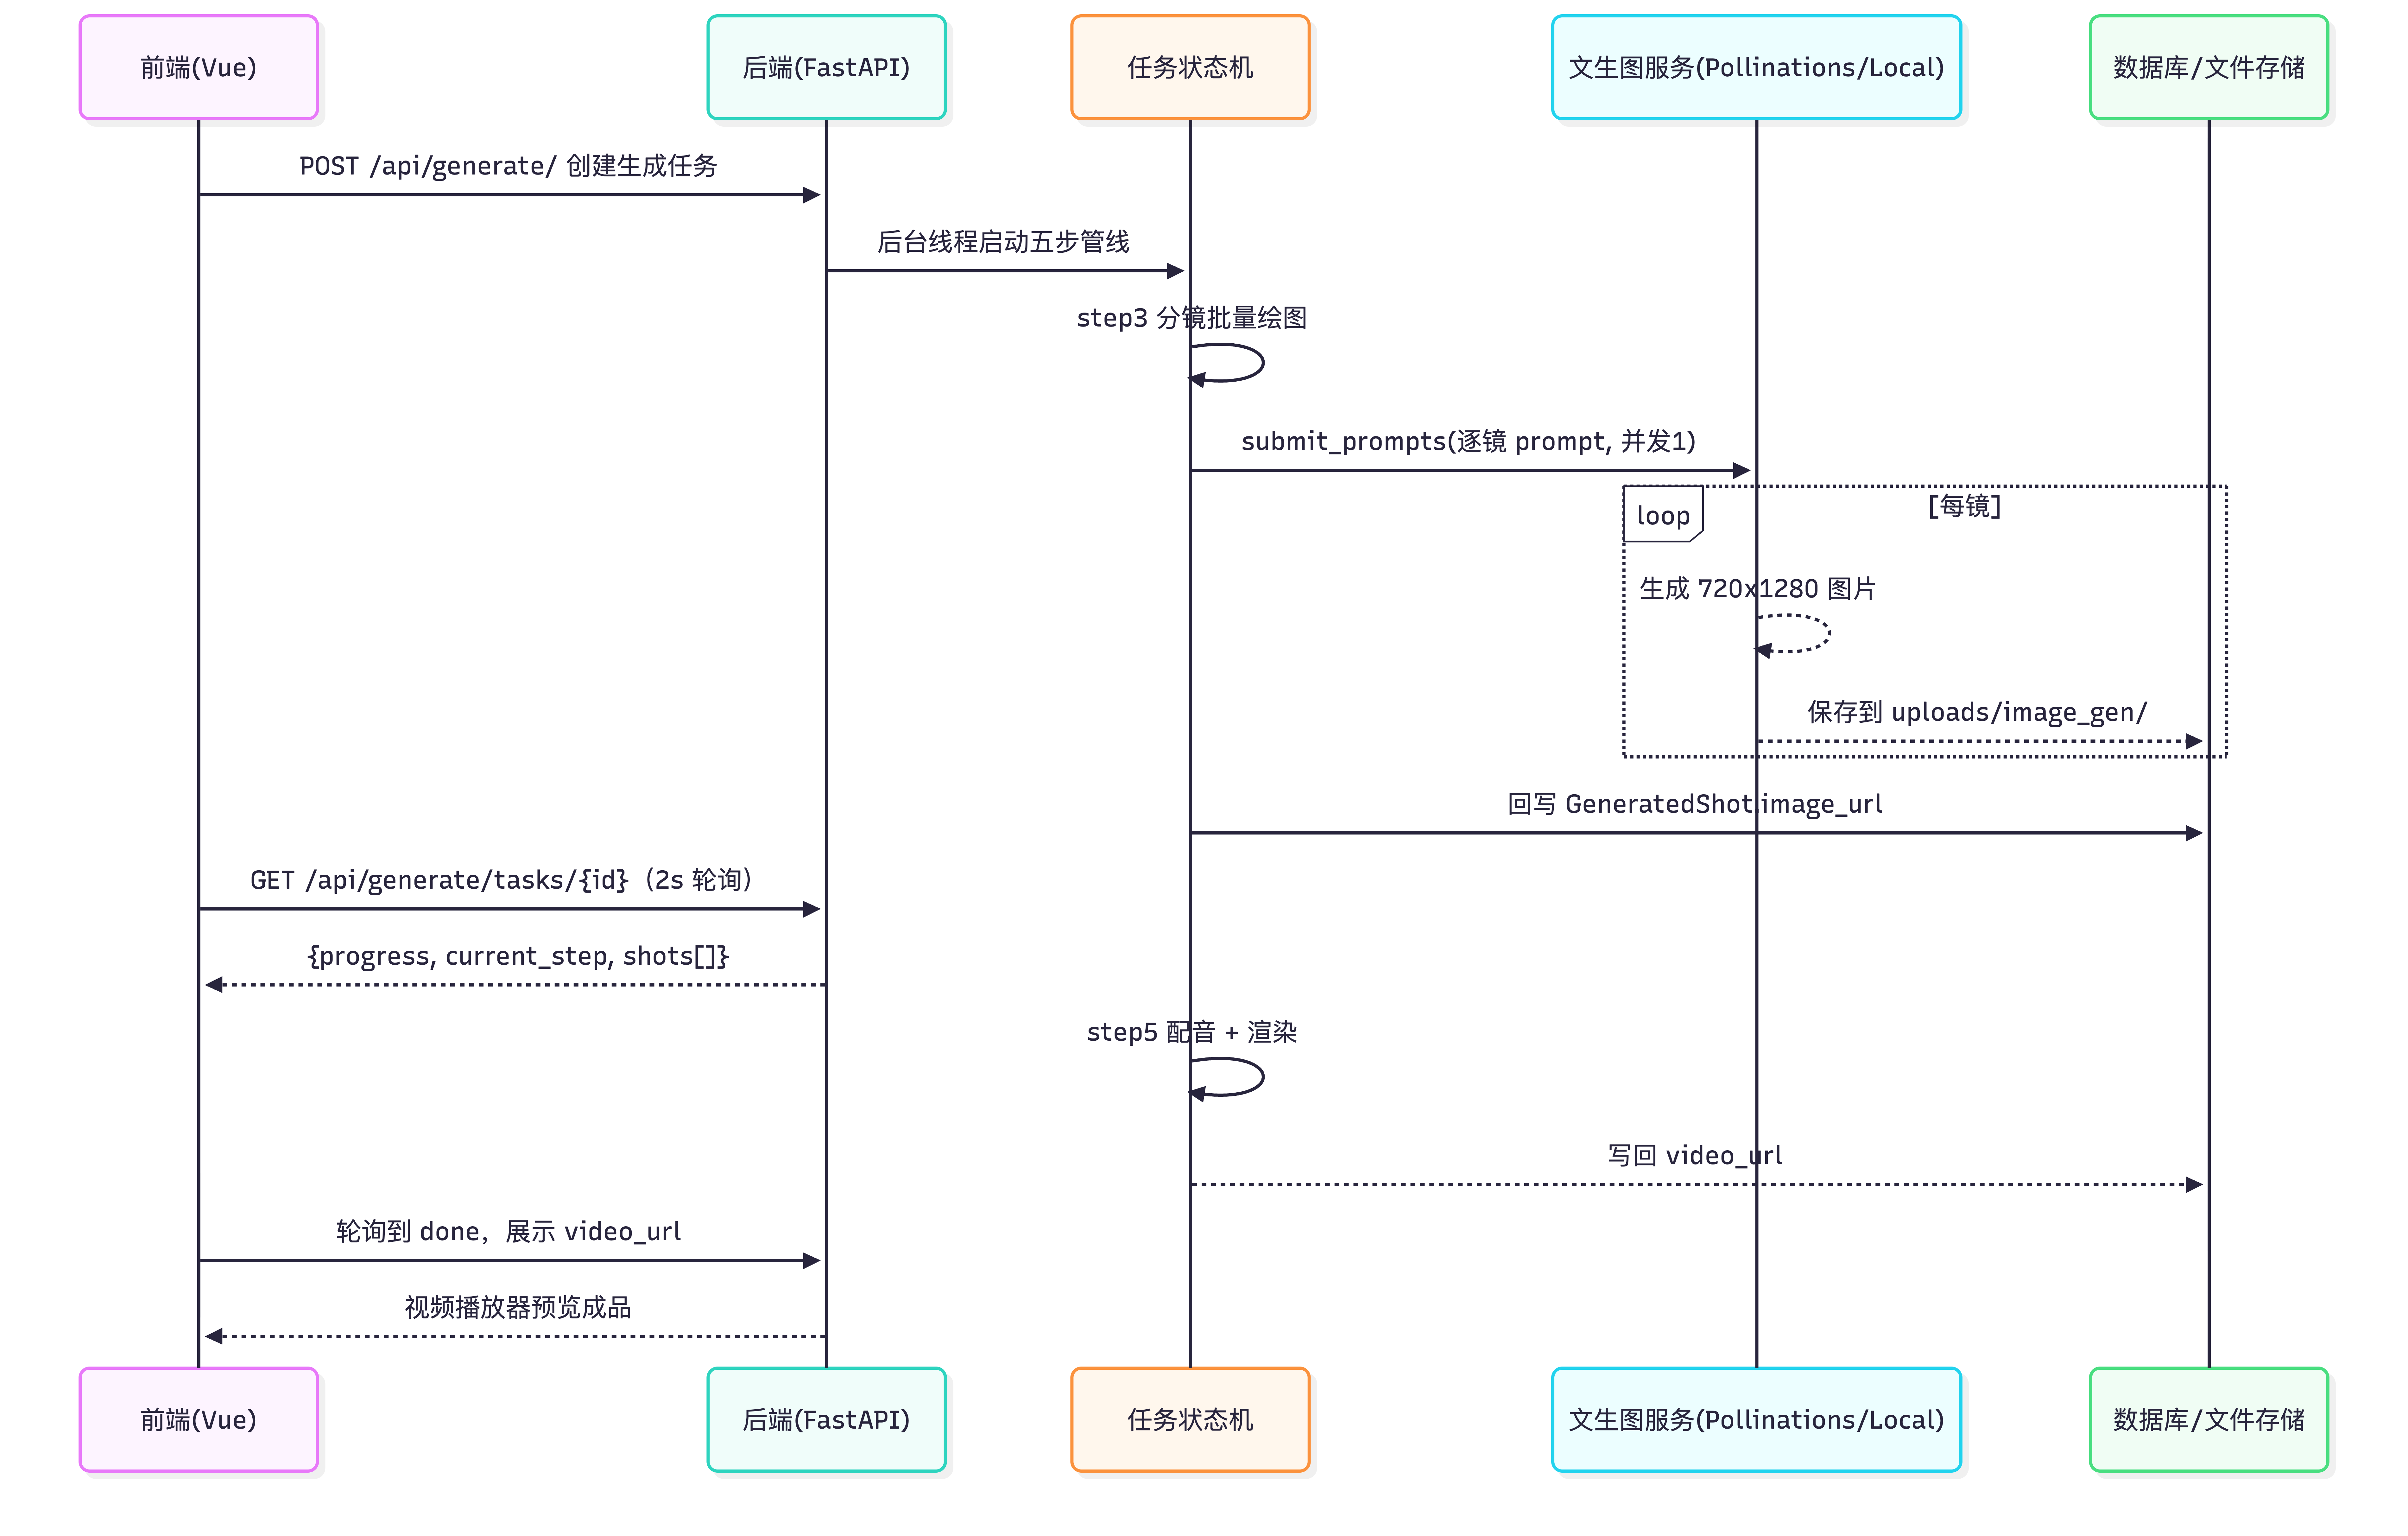
\includegraphics[width=\textwidth]{assets/flow.png}
\caption{核心业务流程数据流向图}\label{fig:flow}
\end{figure}

\textbf{关键流程时序图（"AI 图片批量生成"完整流程）}，如图 \ref{fig:seq}：前端工作台提交生成任务，后台线程通过 BatchImageService 将各镜头并发提交至图像生成服务，逐镜回调更新任务进度，前端轮询直至 status=done、progress=100\%。

\begin{figure}[htbp]
\centering
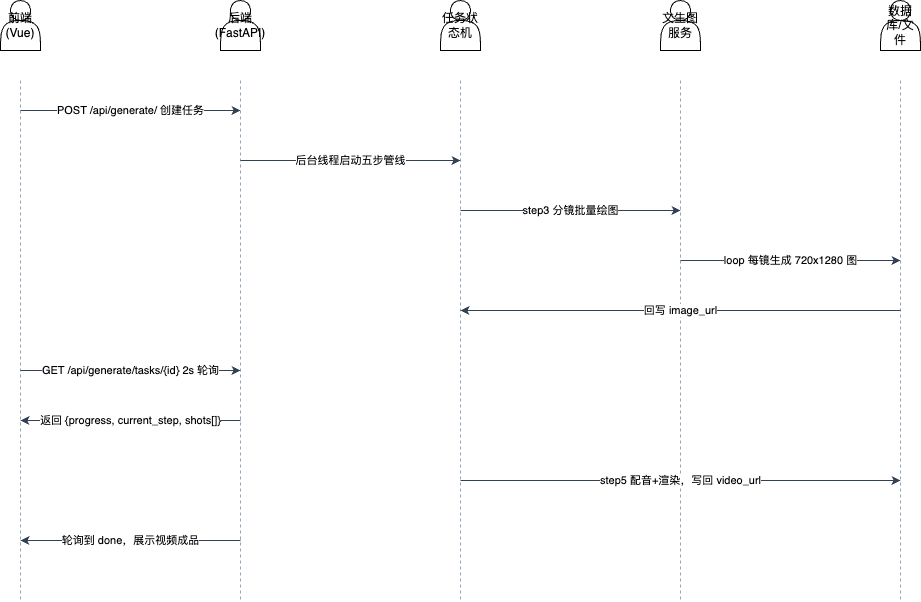
\includegraphics[width=0.95\textwidth]{assets/sequence.png}
\caption{AI 图片批量生成时序图}\label{fig:seq}
\end{figure}

% ============================================================================
\chapter{技术栈说明}
\section{技术栈总览}

\begin{longtable}{p{3cm}p{3.8cm}p{2cm}p{6.2cm}}
\caption{技术栈总览}\label{tab:stack}\\
\toprule
类别 & 技术选型 & 版本 & 选型理由\\
\midrule
\endfirsthead
\toprule
类别 & 技术选型 & 版本 & 选型理由\\
\midrule
\endhead
前端框架 & Vue 3 + Vite & 3.5 / 8.2 & 组合式 API 开发效率高，构建快、代理配置简单\\
前端 UI & Element Plus + ECharts & 2.14 / 6.1 & 组件丰富；ECharts 用于情绪曲线可视化\\
后端框架 & FastAPI + Pydantic v2 & 0.115+ & 自动 OpenAPI 文档、异步支持、类型校验\\
后端 ORM & SQLAlchemy 2.0 & 2.0.40 & 声明式建模，支持 SQLite/MySQL 切换\\
数据库 & SQLite（可切 MySQL） & 内置 / 8.x & 开发零配置；DB\_TYPE 一键切换\\
AI 文本模型 & DeepSeek API & deepseek-chat & 国产模型，长文本分镜生成性价比高\\
图像生成 & 可图 / 可灵（预留） & — & 国产文生图/视频；当前以 Mock 实现\\
语音合成 & Edge-TTS（预留）/ Mock & — & 免费可用；Mock 保证离线可演示\\
视频处理 & FFmpeg + Pillow & 8.1 / 12.3 & FFmpeg 滤镜链合成；Pillow 渲染字幕\\
认证 & PyJWT + bcrypt & 2.10 / 4.2 & JWT Token 认证 + 密码哈希\\
依赖管理 & pip + venv & — & 项目级虚拟环境隔离\\
\bottomrule
\end{longtable}

\section{关键技术说明}

\begin{enumerate}
\item \textbf{LLM 调用方式}：通过 OpenAI 兼容 REST API 调用 DeepSeek（\texttt{llm\_base\_url} 指向 \url{https://api.deepseek.com/v1}），使用 Chat Completions 接口并设计结构化 Prompt 输出 JSON 分镜数据；未配置 \texttt{LLM\_API\_KEY} 时自动降级为内置 Mock 分镜。
\item \textbf{图像生成调度}：\texttt{BaseImageGenerator} 抽象接口 + \texttt{BatchImageService} 线程池调度，用 \texttt{Semaphore} 控制并发上限，避免突发请求打满外部 API。
\item \textbf{TTS 引擎}：\texttt{BaseTTSService} 定义 \texttt{synthesize()} 接口；Mock 实现按「字数 ÷ 4.5 ÷ 情绪系数」估算时长（悲伤最慢、愤怒最快），并生成可访问的假音频 URL。
\item \textbf{视频合成}：\texttt{ffprobe} 探测音频时长 → 计算总帧数 → \texttt{zoompan} 滤镜生成推/拉镜头 → Pillow 渲染字幕 PNG → \texttt{overlay} 滤镜叠加 → \texttt{-t} 截断 + \texttt{-shortest} 兜底，实现时长对齐。
\end{enumerate}

\section{开发环境}

\begin{longtable}{p{4cm}p{11cm}}
\caption{开发环境}\label{tab:env}\\
\toprule
项目 & 配置\\
\midrule
\endfirsthead
\toprule
项目 & 配置\\
\midrule
\endhead
操作系统 & macOS（Apple Silicon）\\
开发语言 & Python 3.14.3、JavaScript (ESM)\\
IDE & VS Code / Trae IDE\\
后端依赖 & \texttt{requirements.txt}（fastapi、uvicorn、sqlalchemy、pillow 等）\\
前端依赖 & \texttt{package.json}（vue、element-plus、axios、pinia、echarts 等）\\
媒体工具 & FFmpeg 8.1.2（brew 安装，含 ffprobe）\\
\bottomrule
\end{longtable}

% ============================================================================
\chapter{数据库表设计}
\section{ER 图（实体关系）}

系统共 12 张业务表，实体关系如图 \ref{fig:er} 所示：

\begin{figure}[htbp]
\centering
\includegraphics[width=0.78\textwidth]{assets/er-diagram.png}
\caption{数据库 ER 图}\label{fig:er}
\end{figure}

关系基数说明：User 与 Project 为 1:N；Template 与 TemplateVariable / TemplateShot 为 1:N；GenerationTask 与 GeneratedShot 为 1:N；User 与 Template 通过 UserFavorite 为 M:N。

\section{数据表清单}

\begin{longtable}{p{4.2cm}p{10.8cm}}
\caption{数据表清单}\label{tab:tables}\\
\toprule
表名 & 用途说明\\
\midrule
\endfirsthead
\toprule
表名 & 用途说明\\
\midrule
\endhead
users & 用户账号（密码哈希、VIP 标记、每日生成次数）\\
projects & 漫剧项目（标题、分类、画风、进度状态）\\
characters & 角色设定（主角/反派/配角、外貌、性格）\\
scenes & 场景设定（室内/室外/自然、时间段、天气）\\
shots & 项目分镜记录（镜头类型、机位、时长、情绪）\\
templates & 漫剧模板（分类、镜头数、情绪曲线、新手友好标记）\\
template\_variables & 模板变量定义（必填/可选、默认值、示例、AI 生成标记）\\
template\_shots & 模板固定分镜（含 \$\{变量\} 脚本模板、情绪强度）\\
generation\_tasks & 生成任务（状态机、进度、变量快照、错误信息）\\
generated\_shots & 任务产出的分镜（脚本内容、图片 URL、状态）\\
assets & 素材资产（上传文件路径、类型、尺寸）\\
user\_favorites & 用户收藏模板关系表\\
\bottomrule
\end{longtable}

\section{核心表结构详细设计}

\textbf{表：users}

\begin{longtable}{p{3.6cm}p{3cm}p{1.6cm}p{1.8cm}p{5cm}}
\caption{users 表结构}\label{tab:users}\\
\toprule
字段名 & 数据类型 & 是否为空 & 默认值 & 说明\\
\midrule
\endfirsthead
\toprule
字段名 & 数据类型 & 是否为空 & 默认值 & 说明\\
\midrule
\endhead
id & Integer PK & 否 & 自增 & 主键\\
username & String(50) & 否 & — & 登录名，唯一\\
email & String(100) & 否 & — & 邮箱，唯一\\
hashed\_password & String(255) & 否 & — & bcrypt 密码哈希\\
nickname & String(50) & 是 & — & 昵称\\
is\_vip & Boolean & 否 & False & 是否 VIP\\
daily\_generate\_count & Integer & 否 & 0 & 每日生成次数\\
\bottomrule
\end{longtable}

设计说明：密码只存哈希不存明文；每日生成次数用于免费用户配额限制（日限 10 次）。

\textbf{表：templates}

\begin{longtable}{p{3.6cm}p{3.2cm}p{1.6cm}p{1.8cm}p{4.8cm}}
\caption{templates 表结构}\label{tab:templates}\\
\toprule
字段名 & 数据类型 & 是否为空 & 默认值 & 说明\\
\midrule
\endfirsthead
\toprule
字段名 & 数据类型 & 是否为空 & 默认值 & 说明\\
\midrule
\endhead
id & Integer PK & 否 & 自增 & 主键\\
template\_code & String(100) & 否 & — & 模板编码，唯一约束\\
name & String(200) & 否 & — & 模板名称\\
category & String(50) & 否 & — & 分类（都市/古风/甜宠/悬疑…）\\
total\_shots & Integer & 否 & 10 & 镜头总数\\
emotion\_curve & JSON & 是 & — & 情绪曲线数组\\
is\_beginner\_friendly & Boolean & 否 & False & 新手友好标记\\
\bottomrule
\end{longtable}

设计说明：情绪曲线与分镜结构以 JSON 存储，灵活支持不同模板的差异化设计，避免为每个模板建表。

\textbf{表：generation\_tasks}

\begin{longtable}{p{3.8cm}p{3.4cm}p{1.6cm}p{1.8cm}p{4.4cm}}
\caption{generation\_tasks 表结构}\label{tab:gen}\\
\toprule
字段名 & 数据类型 & 是否为空 & 默认值 & 说明\\
\midrule
\endfirsthead
\toprule
字段名 & 数据类型 & 是否为空 & 默认值 & 说明\\
\midrule
\endhead
id & Integer PK & 否 & 自增 & 主键\\
user\_id & Integer FK & 否 & — & 归属用户\\
template\_id & Integer FK & 是 & — & 使用的模板\\
task\_type & String(30) & 否 & from\_template & 任务类型\\
status & String(20) & 否 & pending & pending/running/done/failed/cancelled\\
progress & Integer & 否 & 0 & 进度 0-100\\
variables\_snapshot & JSON & 是 & — & 用户填写的变量快照\\
error\_msg & Text & 是 & — & 失败原因\\
\bottomrule
\end{longtable}

设计说明：任务状态机支撑「提交 → 执行 → 完成」的异步流程；变量快照保证任务可追溯、可复现。

\section{建表 SQL（核心表）}

\begin{lstlisting}[language=SQL,caption={建表 SQL（users/templates/generation\_tasks）},label=lst:sql]
-- users：用户表
CREATE TABLE users (
    id INTEGER PRIMARY KEY AUTOINCREMENT,
    username VARCHAR(50) NOT NULL UNIQUE,
    email VARCHAR(100) NOT NULL UNIQUE,
    hashed_password VARCHAR(255) NOT NULL,
    nickname VARCHAR(50),
    is_vip BOOLEAN NOT NULL DEFAULT 0,
    daily_generate_count INTEGER NOT NULL DEFAULT 0,
    created_at DATETIME DEFAULT CURRENT_TIMESTAMP
);

-- templates：模板表
CREATE TABLE templates (
    id INTEGER PRIMARY KEY AUTOINCREMENT,
    template_code VARCHAR(100) NOT NULL UNIQUE,
    name VARCHAR(200) NOT NULL,
    category VARCHAR(50) NOT NULL,
    description TEXT,
    total_shots INTEGER NOT NULL DEFAULT 10,
    total_duration_sec INTEGER NOT NULL DEFAULT 180,
    emotion_curve JSON,
    tags JSON,
    is_beginner_friendly BOOLEAN NOT NULL DEFAULT 0,
    sort_order INTEGER NOT NULL DEFAULT 0,
    created_at DATETIME DEFAULT CURRENT_TIMESTAMP
);

-- generation_tasks：生成任务表（含外键）
CREATE TABLE generation_tasks (
    id INTEGER PRIMARY KEY AUTOINCREMENT,
    user_id INTEGER NOT NULL REFERENCES users(id),
    project_id INTEGER REFERENCES projects(id),
    template_id INTEGER REFERENCES templates(id),
    task_type VARCHAR(30) NOT NULL DEFAULT 'from_template',
    status VARCHAR(20) NOT NULL DEFAULT 'pending',
    progress INTEGER NOT NULL DEFAULT 0,
    current_step VARCHAR(100),
    variables_snapshot JSON,
    error_msg TEXT,
    total_shots INTEGER NOT NULL DEFAULT 0,
    completed_shots INTEGER NOT NULL DEFAULT 0,
    created_at DATETIME DEFAULT CURRENT_TIMESTAMP
);
CREATE INDEX ix_generation_tasks_user_id ON generation_tasks (user_id);
CREATE INDEX ix_generation_tasks_status ON generation_tasks (status);
\end{lstlisting}

% ============================================================================
\chapter{API 接口说明}
\section{接口总览}

\begin{longtable}{p{1.6cm}p{3.6cm}p{1.8cm}p{4.6cm}p{1.6cm}p{1.2cm}}
\caption{API 接口总览}\label{tab:api}\\
\toprule
编号 & 接口名称 & 方法 & 路径 & 模块 & 认证\\
\midrule
\endfirsthead
\toprule
编号 & 接口名称 & 方法 & 路径 & 模块 & 认证\\
\midrule
\endhead
API-01 & 用户登录 & POST & /api/auth/login & 认证 & 否\\
API-02 & 当前用户信息 & GET & /api/auth/me & 认证 & 是\\
API-03 & 项目列表 & GET & /api/projects & 项目 & 是\\
API-04 & 模板列表 & GET & /api/templates & 模板 & 是\\
API-05 & 模板详情 & GET & /api/templates/\{id\} & 模板 & 是\\
API-06 & 创建生成任务 & POST & /api/generate & 生成 & 是\\
API-07 & 任务详情 & GET & /api/generate/tasks/\{id\} & 生成 & 是\\
API-08 & AI 变量补全 & POST & /api/generate/ai-fill-variables & 生成 & 是\\
API-09 & Mock 分镜数据 & GET & /api/script-generator/mock & M1 & 是\\
API-10 & 剧本转分镜 & POST & /api/script-generator/convert & M1 & 是\\
API-11 & 音色列表 & GET & /api/tts/voices & M3 & 是\\
API-12 & 生成配音 & POST & /api/tts/generate & M3 & 是\\
API-13 & 提交图片生成 & POST & /api/image-generator/submit & M2 & 是\\
API-14 & 查询生成任务 & GET & /api/image-generator/tasks/\{id\} & M2 & 是\\
API-15 & 批量提交分镜绘图 & POST & /api/image-generator/batch/submit & M2 & 是\\
API-16 & 批量任务状态 & GET & /api/image-generator/batch/\{id\} & M2 & 是\\
API-17 & 视频合成 & POST & /api/video/compose & M4 & 是\\
\bottomrule
\end{longtable}

\section{接口详细说明（示例）}

\textbf{接口名称}：视频合成（API-17）\\
\textbf{功能描述}：将上传的静态图片、配音音频与台词文本合成为带 Ken Burns 效果与字幕烧录的视频片段。\\
\textbf{请求方法与路径}：\texttt{POST /api/video/compose}（multipart/form-data）

请求参数如表 \ref{tab:compose-params}：

\begin{table}[htbp]
\centering
\begin{tabular}{p{3.2cm}p{2.6cm}p{2.2cm}p{6.4cm}}
\toprule
参数名 & 类型 & 是否必填 & 说明\\
\midrule
image & File & 是 & 静态图片\\
audio & File & 是 & 配音音频\\
subtitle\_text & Form String & 否 & 台词字幕文本（空则不烧字幕）\\
width / height & Form Int & 否 & 输出分辨率，默认 1080x1920\\
direction & Form String & 否 & Ken Burns 方向：in 推近 / out 拉远，默认 in\\
\bottomrule
\end{tabular}
\caption{视频合成请求参数}\label{tab:compose-params}
\end{table}

请求示例：

\begin{lstlisting}[language=bash,caption={视频合成请求示例},label=lst:compose]
curl -X POST http://localhost:8000/api/video/compose \
  -F "image=@scene.png" -F "audio=@voice.wav" \
  -F "subtitle_text=三年之期已满，龙神归位！" -F "direction=in"
\end{lstlisting}

响应示例（成功）：

\begin{lstlisting}[caption={视频合成成功响应},label=lst:compose-ok]
{ "video_url": "/uploads/video_out/274e133c13.mp4", "duration": 4.2 }
\end{lstlisting}

响应示例（失败）：

\begin{lstlisting}[caption={视频合成失败响应},label=lst:compose-fail]
{ "detail": "图片文件不存在: /nonexistent_scene.png" }
\end{lstlisting}

\textbf{状态码说明}：200 成功；400 输入文件缺失或参数错误；500 FFmpeg 合成失败（错误信息含 stderr 摘要）。

\section{接口规范}

\begin{enumerate}
\item \textbf{统一前缀与文档}：全部接口以 /api 为前缀；Swagger 文档位于 \url{http://localhost:8000/api/docs}。
\item \textbf{统一响应格式}：业务接口直接返回数据对象；错误统一返回 \texttt{\{"detail": "错误描述"\}}，前端 Axios 拦截器统一提取 detail 并弹出提示。
\item \textbf{认证机制}：生产模式采用 JWT Bearer Token——登录返回 \texttt{access\_token}，前端存入 localStorage，请求拦截器自动附加 \texttt{Authorization: Bearer <token>}；开发模式认证关闭，无 Token 时返回默认 admin 用户，便于演示。
\item \textbf{文件类接口}：图片/音频/视频上传与合成均使用 multipart/form-data；产物通过 /uploads 静态路径访问。
\end{enumerate}

% ============================================================================
\chapter{项目实现方法}
\section{实现概述}

项目按「先搭骨架、再填模块」的顺序实现：先搭建 FastAPI 后端骨架（配置、数据库、路由注册）与 Vue 前端骨架（布局、路由、API 封装），随后按 M1→M4 依次实现四大模块，最后以 \texttt{generate} 任务状态机将模块串联为完整流水线。所有 AI 能力均通过抽象接口实现并附带 Mock 降级，保证在无外部 API Key 的情况下全流程可演示。

\section{M1 模块：AI 剧本与分镜脚本生成}

\textbf{实现思路}：分镜脚本采用结构化数据结构（Scene：scene\_id/bg\_prompt/character\_prompts/camera\_angle；Dialogue：speaker/line/emotion），由 \texttt{ScriptGeneratorService} 统一产出。有 LLM Key 时调用 DeepSeek 生成，无 Key 时降级 \texttt{generate\_script\_mock()} 返回内置 6 镜完整分镜。模板生成路径则由 \texttt{\_render\_template\_script()} 将 \$\{变量\} 替换为实际值。

\textbf{核心流程}：模板变量输入 → 渲染模板脚本 → 生成分镜 → 入库。

\textbf{关键代码}（变量渲染）：

\begin{lstlisting}[language=Python,caption={模板变量渲染},label=lst:m1]
def _render_template_script(script_template: str, variables: dict) -> str:
    """Replace ${variable} with actual values"""
    def replacer(match):
        key = match.group(1)
        return str(variables.get(key, f"[{key}]"))
    return re.sub(r"\$\{(\w+)\}", replacer, script_template or "")
\end{lstlisting}

\textbf{第三方服务调用（Prompt 设计）}：调用 DeepSeek Chat Completions 接口，系统提示词要求模型"只输出 JSON"，并以 Few-shot 示例约束分镜结构（镜头类型、机位、时长、情绪强度），提高解析成功率；\texttt{parse\_llm\_response} 对返回内容做容错解析（提取 JSON 片段、处理格式偏差）。

\section{M2 模块：分镜图片生成调度}

\textbf{实现思路}：\texttt{BaseImageGenerator} 抽象接口定义 \texttt{submit\_task()/get\_result()}；\texttt{MockImageGenerator} 用后台线程模拟真实生成耗时；\texttt{BatchImageService} 以 \texttt{ThreadPoolExecutor(8)} 提交每镜任务、\texttt{Semaphore(concurrency)} 限制并发数，并对每镜任务轮询直到 completed/failed。

\textbf{核心流程}：提交分镜脚本 → 创建 BatchJob → 并发提交各镜 → 每镜完成回调更新 → 前端轮询批量状态。

\textbf{关键代码}（批量并发调度）：

\begin{lstlisting}[language=Python,caption={批量并发调度（app/services/image\_gen/batch.py）},label=lst:m2]
# 并发提交：每个镜头一个 worker，受信号量约束，避免瞬时打爆生成服务
semaphore = Semaphore(max(1, concurrency))

def _worker(item: BatchTaskItem, scene) -> None:
    with semaphore:
        task = ImageTask(
            scene_id=item.scene_id,
            prompt=self._build_prompt(scene, resolved_style),
            negative_prompt=DEFAULT_NEGATIVE,
            style=resolved_style,
            aspect_ratio=aspect_ratio,
        )
        task_id = self.generator.submit_task(task)
        item.task_id = task_id
        self._update(batch_id, item.scene_id, status="generating")
        # 轮询直到单任务结束
        while True:
            result = self.generator.get_result(task_id)
            if result.status == "completed":
                self._update(batch_id, item.scene_id, status="completed", url=result.image_url)
                return
            if result.status == "failed":
                self._update(batch_id, item.scene_id, status="failed",
                             error=result.error or "生成失败")
                return
            time.sleep(0.5)

for item, shot in zip(job.tasks, script.shots):
    self._executor.submit(_worker, item, shot.scene)
return batch_id
\end{lstlisting}

\section{M3 模块：配音合成}

\textbf{实现思路}：\texttt{BaseTTSService} 定义抽象接口，\texttt{MockTTSService} 按台词字数与情绪系数估算时长并生成假音频 URL（/uploads/mock\_tts/...mp3）；\texttt{edge\_tts.py} 预留真实引擎接入位。情绪与语速的关系满足产品预期：悲伤最慢、平静居中、愤怒最快。

\textbf{关键代码}（情绪驱动时长估算）：

\begin{lstlisting}[language=Python,caption={情绪驱动时长估算（app/services/tts/mock.py）},label=lst:m3]
@staticmethod
def _estimate_duration(text: str, emotion: str) -> float:
    base = len(text) / CHARS_PER_SECOND   # CHARS_PER_SECOND = 4.5 中文正常语速
    base /= EMOTION_SPEED_FACTORS.get(emotion, 1.0)  # 愤怒1.2快 / 悲伤0.85慢
    digest = int(hashlib.md5(text.encode("utf-8")).hexdigest(), 16)
    jitter = 0.92 + (digest % 17) / 100   # 基于文本哈希的伪随机抖动 0.92~1.08
    return base * jitter
\end{lstlisting}

\section{M4 模块：视频合成与剪辑}

\textbf{实现思路}：\texttt{VideoComposer} 封装 FFmpeg 调用，核心目标有三：时长严格对齐、Ken Burns 动态效果、字幕烧录。由于本机 brew 版 FFmpeg 未编译 drawtext/subtitles 滤镜，最终采用「Pillow 渲染字幕 PNG + overlay 叠加」方案，兼容任何精简版 FFmpeg。

\textbf{核心流程}：ffprobe 探测音频时长 → 计算总帧数 → 构建滤镜链（scale → crop → zoompan → overlay）→ -t 截断 + -shortest 兜底 → 输出 mp4。

\textbf{关键代码}（滤镜链构建）：

\begin{lstlisting}[language=Python,caption={视频合成滤镜链},label=lst:m4]
total_frames = max(2, round(duration * self.FPS))
zoom = f"1.0+0.15*on/({total_frames}-1)"  # in: 推近 1.0 -> 1.15

kenburns = (
    f"[0:v]scale={width}:{height}:force_original_aspect_ratio=increase,"
    f"crop={width}:{height},"
    f"zoompan=z='{zoom}':x='iw/2-(iw/zoom/2)':y='ih/2-(ih/zoom/2)':"
    f"d={total_frames}:s={width}x{height}:fps={self.FPS}"
)
# 字幕 PNG 作为第二路输入，overlay 叠加到底部居中
vf = f"{kenburns}[v0];[v0][1:v]overlay=x=(W-w)/2:y=H-h-120:eof_action=repeat[v]"
\end{lstlisting}

\textbf{字幕渲染}：Pillow 以 RGBA 透明画布绘制白字黑描边、单行居中、自动换行（最多 3 行截断），再裁剪为紧贴文字的 PNG，最后由 overlay 放置在底部居中位置。

\section{模块集成}

四个模块通过 \texttt{generate} 路由的\textbf{步骤化任务状态机}串联为完整流水线，五大步骤依次为：变量注入模板 → 剧本自动合成（M1）→ 角色图生成（M2）→ 分镜批量绘图（M2）→ 配音合成+渲染（M3/M4）。任务执行在后台线程中推进 current\_step 与 progress，前端每 2s 轮询任务详情刷新进度；任意步骤异常会将任务置为 failed 并记录 error\_msg，保证流程可观测、可恢复。

% ============================================================================
\chapter{测试与验证}
\section{测试方案}

\begin{itemize}
\item \textbf{测试策略}：功能测试（四大模块逐功能点验证）+ 接口测试（curl 调用验证）+ 自动化断言测试（视频合成专项）。
\item \textbf{测试环境}：macOS 本地；后端 uvicorn 8000 端口、前端 Vite 5173 端口；测试数据为 ffmpeg 生成的 testsrc 图片与 5.3s 正弦音频。
\item \textbf{自动化测试}：\texttt{backend/tests/} 下三个独立用例脚本，覆盖时长对齐、Ken Burns 动态与字幕烧录、异常处理。
\end{itemize}

\section{测试用例}

\begin{longtable}{p{1.6cm}p{1.4cm}p{4.4cm}p{4.4cm}p{2.4cm}p{1.2cm}}
\caption{测试用例清单}\label{tab:cases}\\
\toprule
编号 & 模块 & 测试场景 & 预期结果 & 实际结果 & 通过\\
\midrule
\endfirsthead
\toprule
编号 & 模块 & 测试场景 & 预期结果 & 实际结果 & 通过\\
\midrule
\endhead
TC-01 & M1 & 调用 Mock 分镜接口 & 返回 6 镜完整结构 & 返回 6 镜 JSON & 通过\\
TC-02 & M1 & 模板变量注入渲染 & 变量被替换为实际值 & 正确替换 & 通过\\
TC-03 & M2 & 提交单镜生成任务 & 返回 task\_id & 正常返回 & 通过\\
TC-04 & M2 & 批量提交 6 镜绘图 & 全部 completed，100\% & 全部完成 & 通过\\
TC-05 & M3 & 查询音色列表 & 返回多音色 & 正常返回 & 通过\\
TC-06 & M3 & 三种情绪配音时长 & 悲伤>平静>愤怒 & 12.4>10.6>8.8s & 通过\\
TC-07 & M4 & 推镜头合成 & 偏差 < 0.1s & 20ms & 通过\\
TC-08 & M4 & 拉镜头合成 & 时长对齐 & 20ms & 通过\\
TC-09 & M4 & 相邻帧差分 & 帧间存在像素差异 & 平均差 7.49 & 通过\\
TC-10 & M4 & 字幕烧录验证 & 底部有白色文字像素 & 6599 个 & 通过\\
TC-11 & M4 & 缺少图片/音频字段上传 & 返回 422 参数校验错误 & 正确返回 & 通过\\
TC-12 & 集成 & 模板一键生成任务 & 状态机走完 5 步 done & 全部完成 & 通过\\
\bottomrule
\end{longtable}

\section{测试结果}

\begin{itemize}
\item 四大模块 12 项用例全部通过；视频合成专项自动化断言（时长偏差 < 0.1s、字幕像素级验证、异常分支）全部通过。
\item 接口测试使用 curl 完成（成功与失败两种响应均已验证）。
\item 已知缺陷/待优化：视频合成为同步执行，超长片段耗时长，后续可接入任务队列异步化；真实 AI 引擎（可图/可灵/Edge-TTS）尚未接入，当前为 Mock 数据。
\end{itemize}

% ============================================================================
\chapter{问题与解决方案}

\paragraph{问题 1：Python 3.14 环境下的依赖兼容问题}
\begin{itemize}
\item \textbf{问题描述}：安装依赖时多个库报错或导入失败（python-jose 停止维护、passlib 与新版 cryptography 冲突）。
\item \textbf{原因分析}：Python 3.14 较新，大量旧版依赖未适配；部分库长期未维护。
\item \textbf{解决过程}：python-jose 替换为 PyJWT（调整 security.py 的 import 与 decode）；移除 passlib 改用 bcrypt 直接调用；requirements.txt 全部升级至兼容 3.14 的版本。
\item \textbf{经验总结}：新版本 Python 生态适配应先冒烟验证关键依赖再写业务代码；长期未维护的库应尽早替换。
\end{itemize}

\paragraph{问题 2：前端 401 未提供认证令牌}
\begin{itemize}
\item \textbf{问题描述}：前端所有业务请求返回 401，页面无法使用。
\item \textbf{原因分析}：后端强制校验 Token，演示阶段用户未登录，前端拦截器自动跳转登录页形成死循环。
\item \textbf{解决过程}：开发模式改为"无 Token 返回默认 admin 用户"，前端路由守卫直接放行；保留登录页与 401 跳转逻辑以便恢复生产鉴权。
\item \textbf{经验总结}：鉴权应区分开发/生产模式，通过配置开关切换，避免阻塞业务流程验证。
\end{itemize}

\paragraph{问题 3：brew 版 FFmpeg 缺少字幕滤镜}
\begin{itemize}
\item \textbf{问题描述}：视频合成报错 \texttt{No such filter: 'drawtext'}（此前 subtitles 同样不可用）。
\item \textbf{原因分析}：Homebrew 精简编译的 FFmpeg 未包含 libfreetype/libass，文字类滤镜缺失。
\item \textbf{解决过程}：改用「Pillow 渲染透明字幕 PNG + overlay 叠加」方案，实测中文渲染正常、兼容精简版 FFmpeg。
\item \textbf{经验总结}：依赖系统二进制能力前应先探测能力矩阵（\texttt{ffmpeg -filters}），选择兼容性最强的实现路径。
\end{itemize}

\paragraph{问题 4：TTS 情绪时长方向错误}
\begin{itemize}
\item \textbf{问题描述}：最初"愤怒"配音时长（12.67s）反而比"平静"（10.56s）更长，与产品预期相反。
\item \textbf{原因分析}：时长估算将情绪系数放在乘法位置（系数越大时长越长），而预期是愤怒语速快、时长短。
\item \textbf{解决过程}：将系数从乘法改为除法（字数 / 4.5 / 系数），愤怒 8.8s < 平静 10.6s < 悲伤 12.4s。
\item \textbf{经验总结}：涉及"越大/越小"方向的参数，应建立清晰语义映射并在用例中固化验证（TC-06）。
\end{itemize}

% ============================================================================
\chapter{创新点}
\section{创新点列举}

\begin{enumerate}
\item 模板驱动的漫剧批量生产方案（功能/产品创新）
\item 基于 Pillow + overlay 的轻量字幕烧录方案（工程创新）
\item 可插拔的 AI 服务抽象架构（架构创新）
\item 步骤化任务状态机 + 前端轮询的异步编排（架构/工程创新）
\end{enumerate}

\section{创新点详述}

\paragraph{创新点 1：模板驱动的批量生产}
\textbf{创新之处}：将"情绪曲线 + 分镜结构 + 变量体系"封装为可复用模板，创作者只需填 2--4 个必填变量即可量产。\\
\textbf{实现方式}：模板表存储分镜脚本模板（含 \$\{变量\} 占位符）与情绪曲线 JSON，生成时经 \texttt{\_render\_template\_script} 注入变量。\\
\textbf{价值}：新人上手门槛显著降低（模板工作台 3 步即可完成一次生成）；成片质量下限由模板情绪节奏保证。对比自由创作类工具，本项目更贴合短剧团队的批量生产诉求。

\paragraph{创新点 2：Pillow + overlay 字幕烧录方案}
\textbf{创新之处}：不依赖 FFmpeg 的 drawtext/subtitles 滤镜（精简版常缺失），改用图像渲染 + 滤镜叠加实现字幕。\\
\textbf{实现方式}：Pillow 渲染 RGBA 字幕 PNG（自动换行、描边、居中），作为第二路输入经 overlay 叠加；时长与位置完全可控。\\
\textbf{价值}：兼容任何 FFmpeg 发行版，避免重装/自编译成本；中文渲染质量优于 drawtext 对字体的依赖。

\paragraph{创新点 3：可插拔 AI 服务抽象架构}
\textbf{创新之处}：LLM、TTS、图像生成均通过抽象接口（BaseTTSService/BaseImageGenerator）隔离，Mock 与真实引擎可随时切换。\\
\textbf{实现方式}：工厂函数按配置（tts\_engine 等）实例化具体实现；未配置 Key 自动降级 Mock。\\
\textbf{价值}：无 Key 可完整演示全流程；接入真实厂商只需新增实现类，不改动业务代码，契合"国产大模型生态"技术路线。

\paragraph{创新点 4：步骤化任务状态机 + 轮询}
\textbf{创新之处}：生成任务以五步状态机推进（变量注入→剧本→角色图→分镜绘图→配音渲染），每步更新 current\_step 与 progress。\\
\textbf{实现方式}：后台线程执行 + 前端每 2s 轮询任务详情，UI 实时展示步骤勾选态。\\
\textbf{价值}：长耗时流程对用户完全透明可观测，对比"一键黑盒"体验更专业，也更便于定位失败环节。

% ============================================================================
\chapter{成果展示与截图}
\section{功能演示截图}

以下均为项目实际运行画面截图（图 \ref{fig:shot-home} ~ 图 \ref{fig:shot-video}），覆盖从首页到成品的完整流程：

\begin{figure}[htbp]
\centering
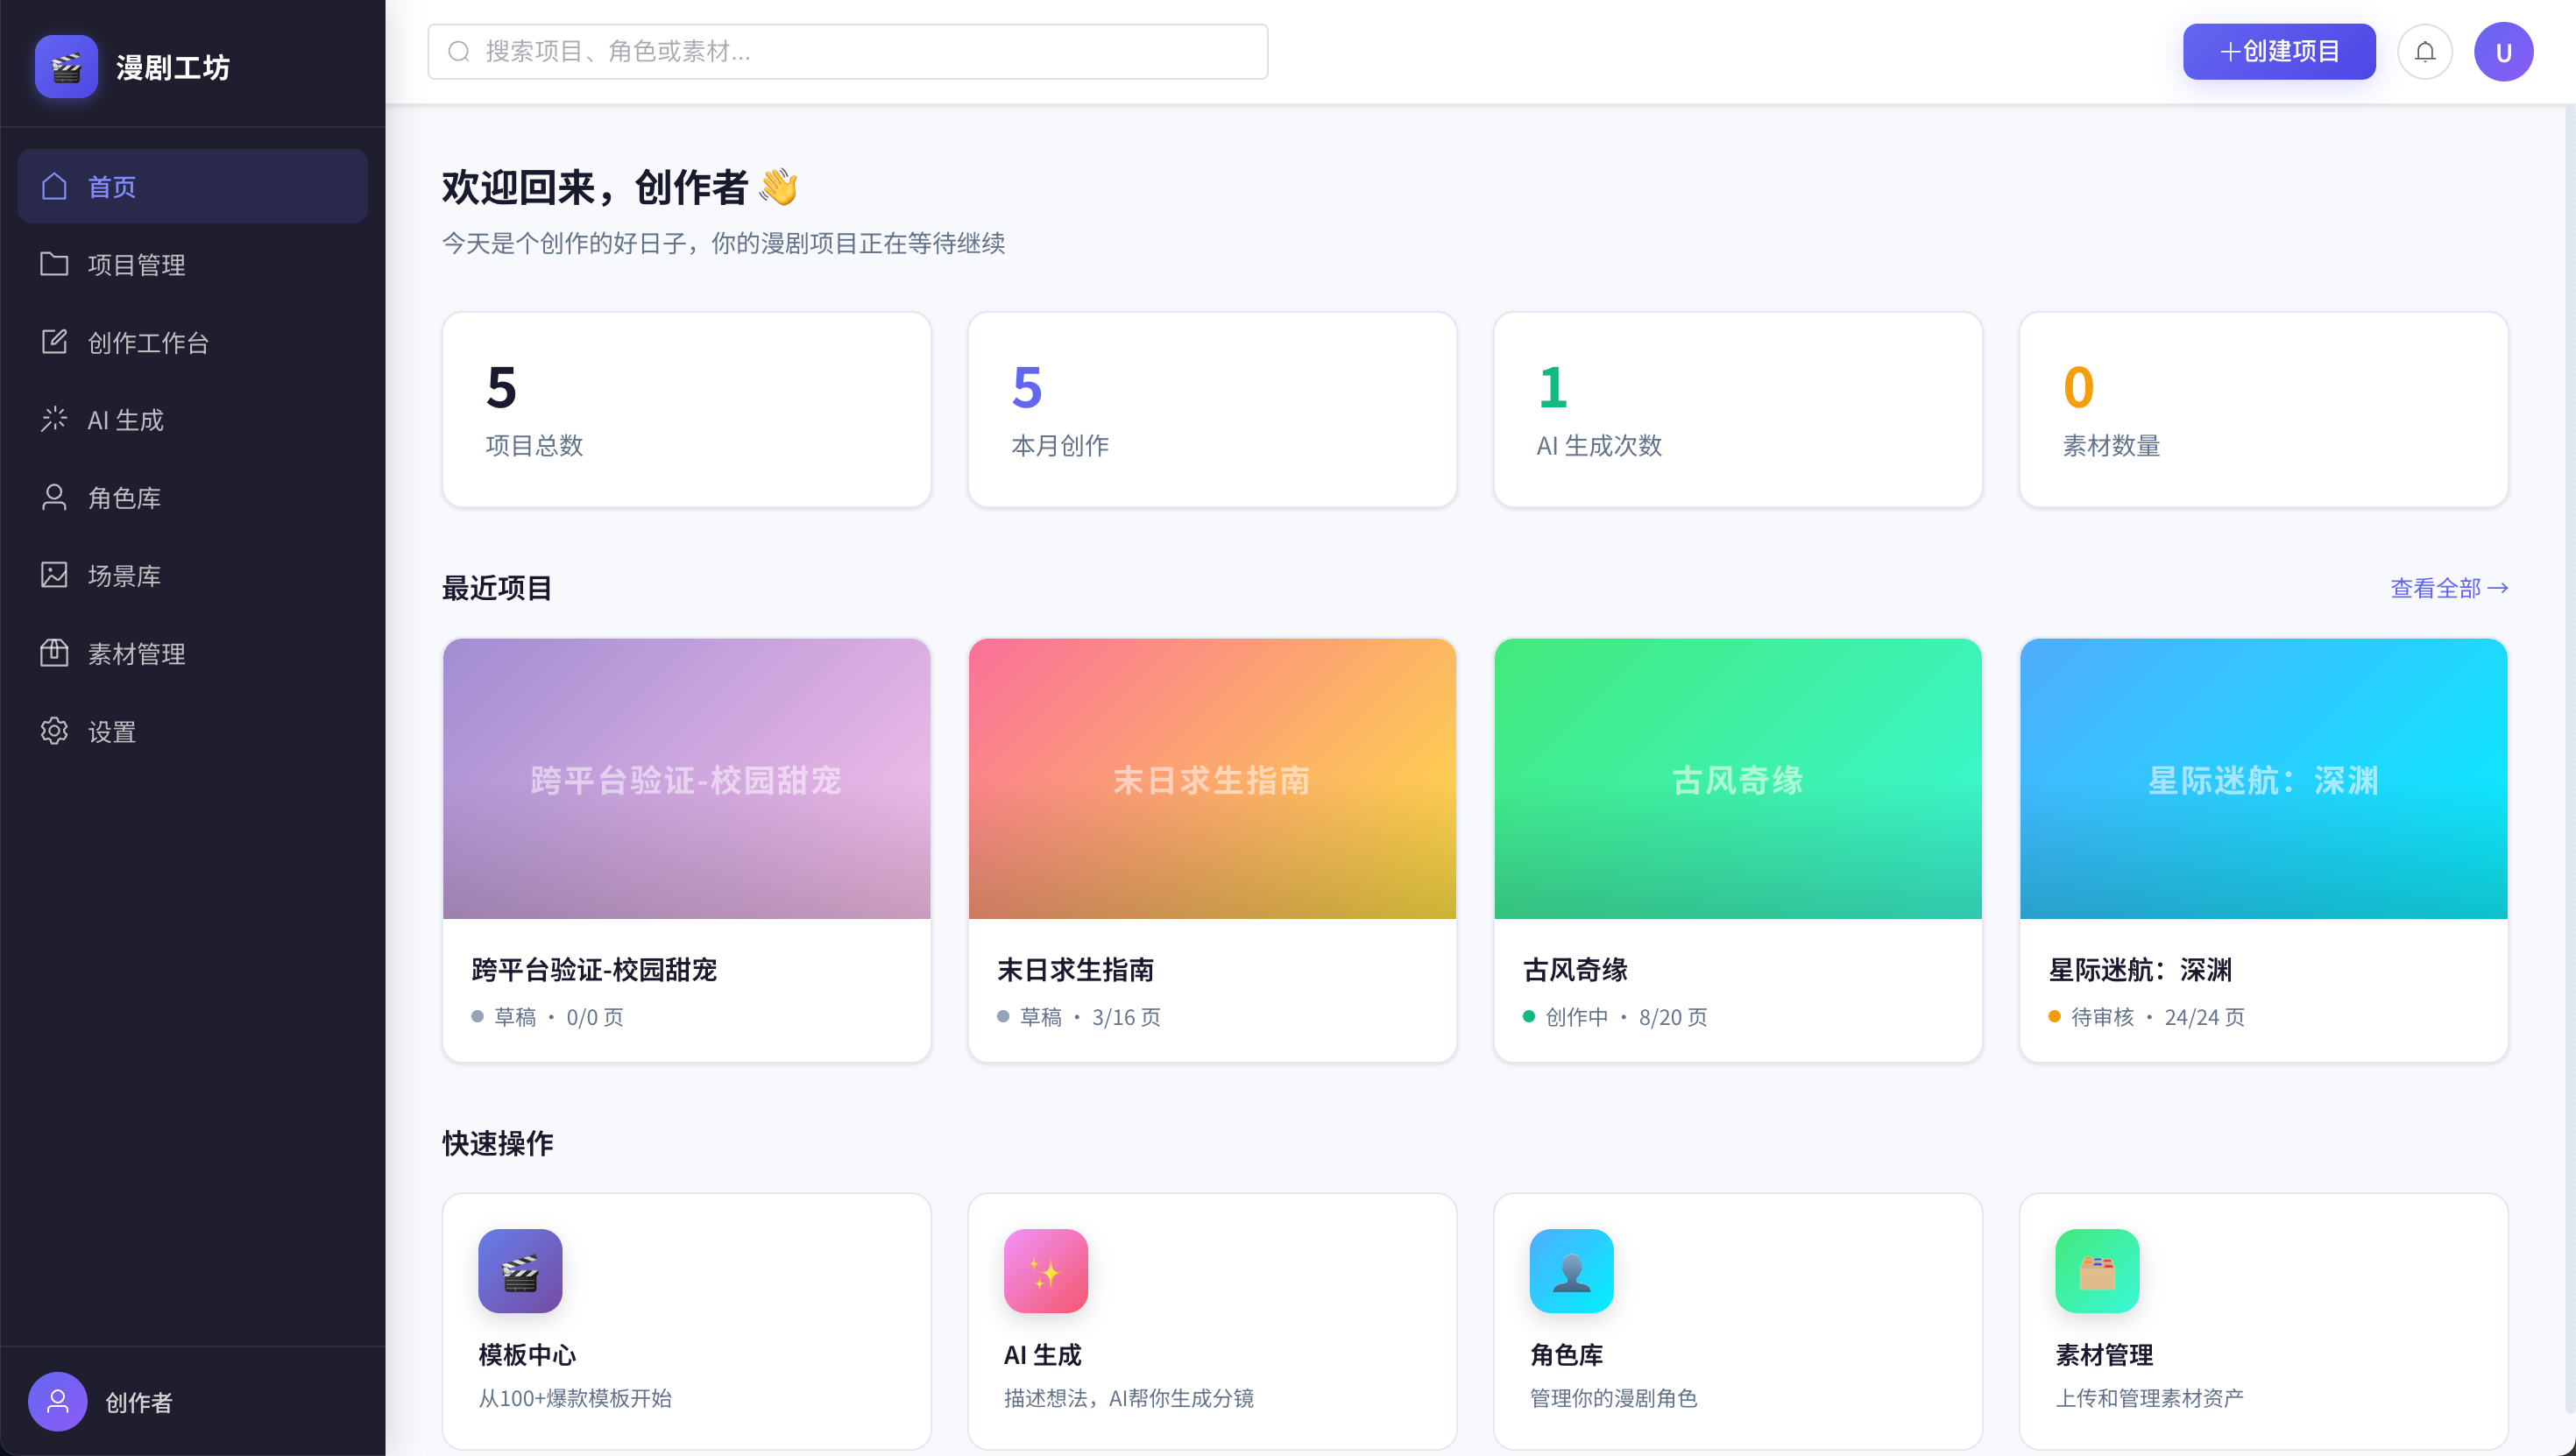
\includegraphics[width=0.88\textwidth]{assets/shot-home.png}
\caption{平台首页（模板推荐与一键生成入口）}\label{fig:shot-home}
\end{figure}

\begin{figure}[htbp]
\centering
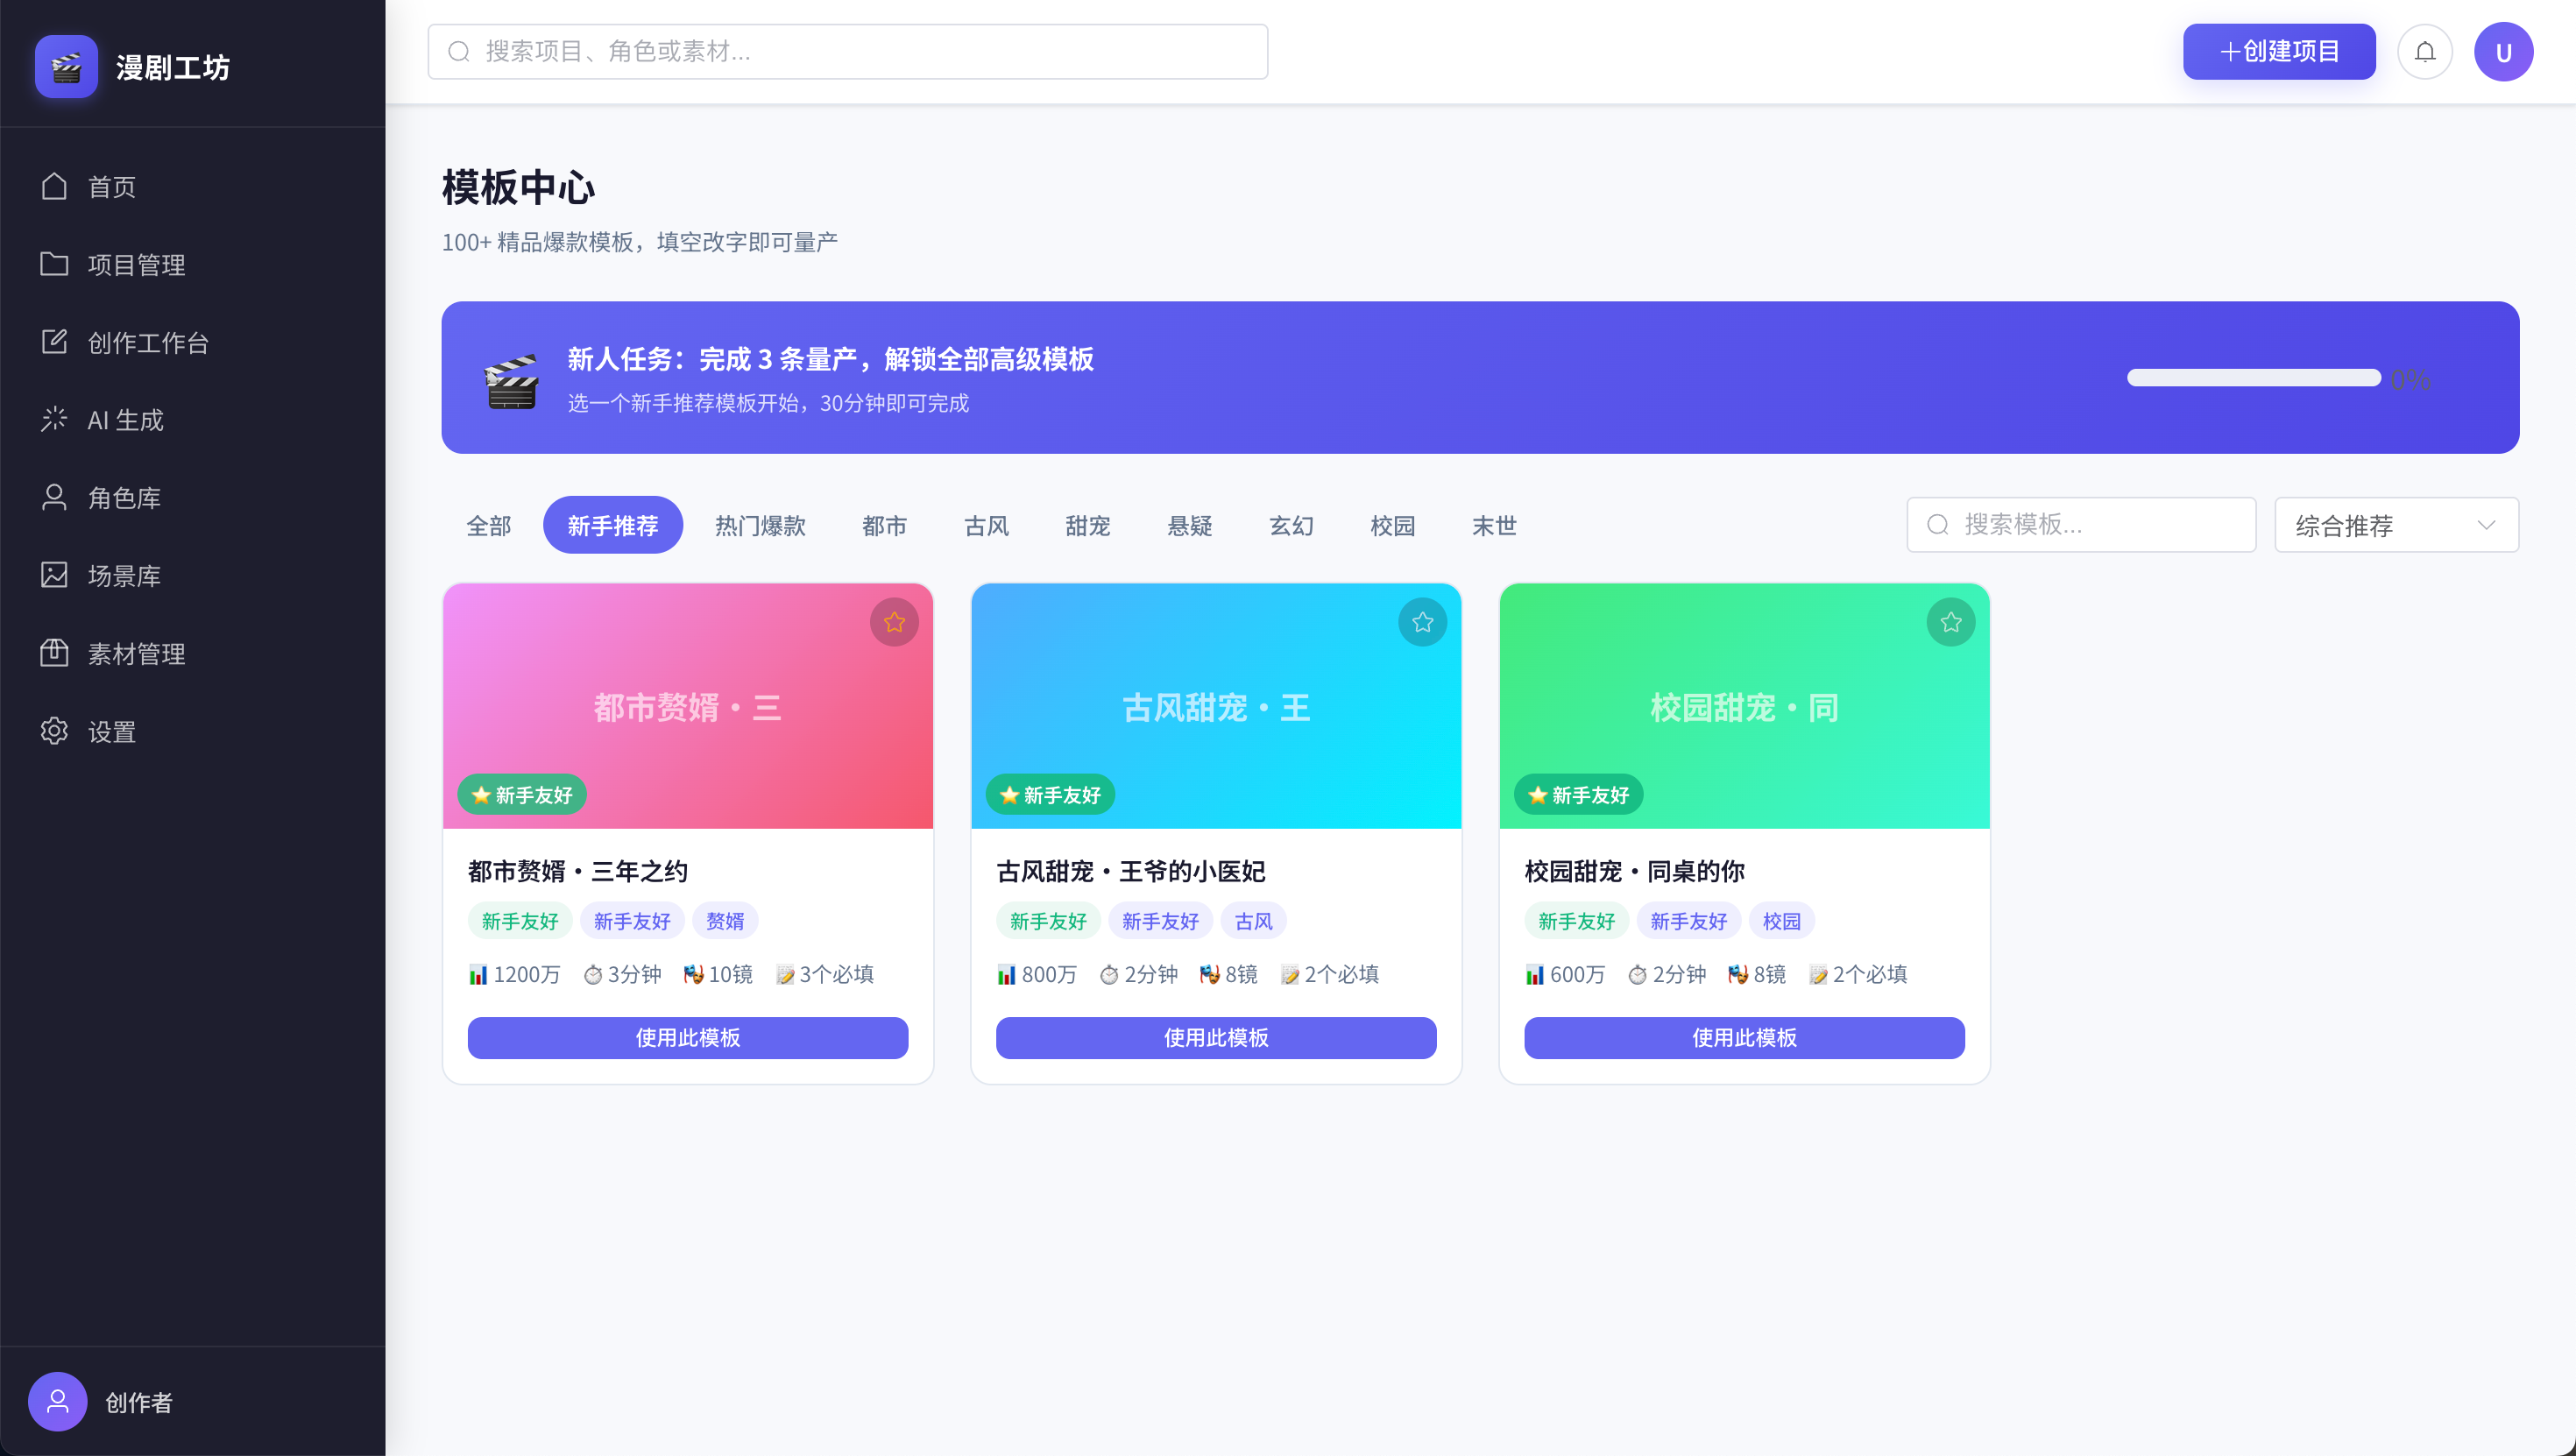
\includegraphics[width=0.88\textwidth]{assets/shot-template.png}
\caption{模板中心（分类筛选与新手友好标记）}\label{fig:shot-template}
\end{figure}

\begin{figure}[htbp]
\centering
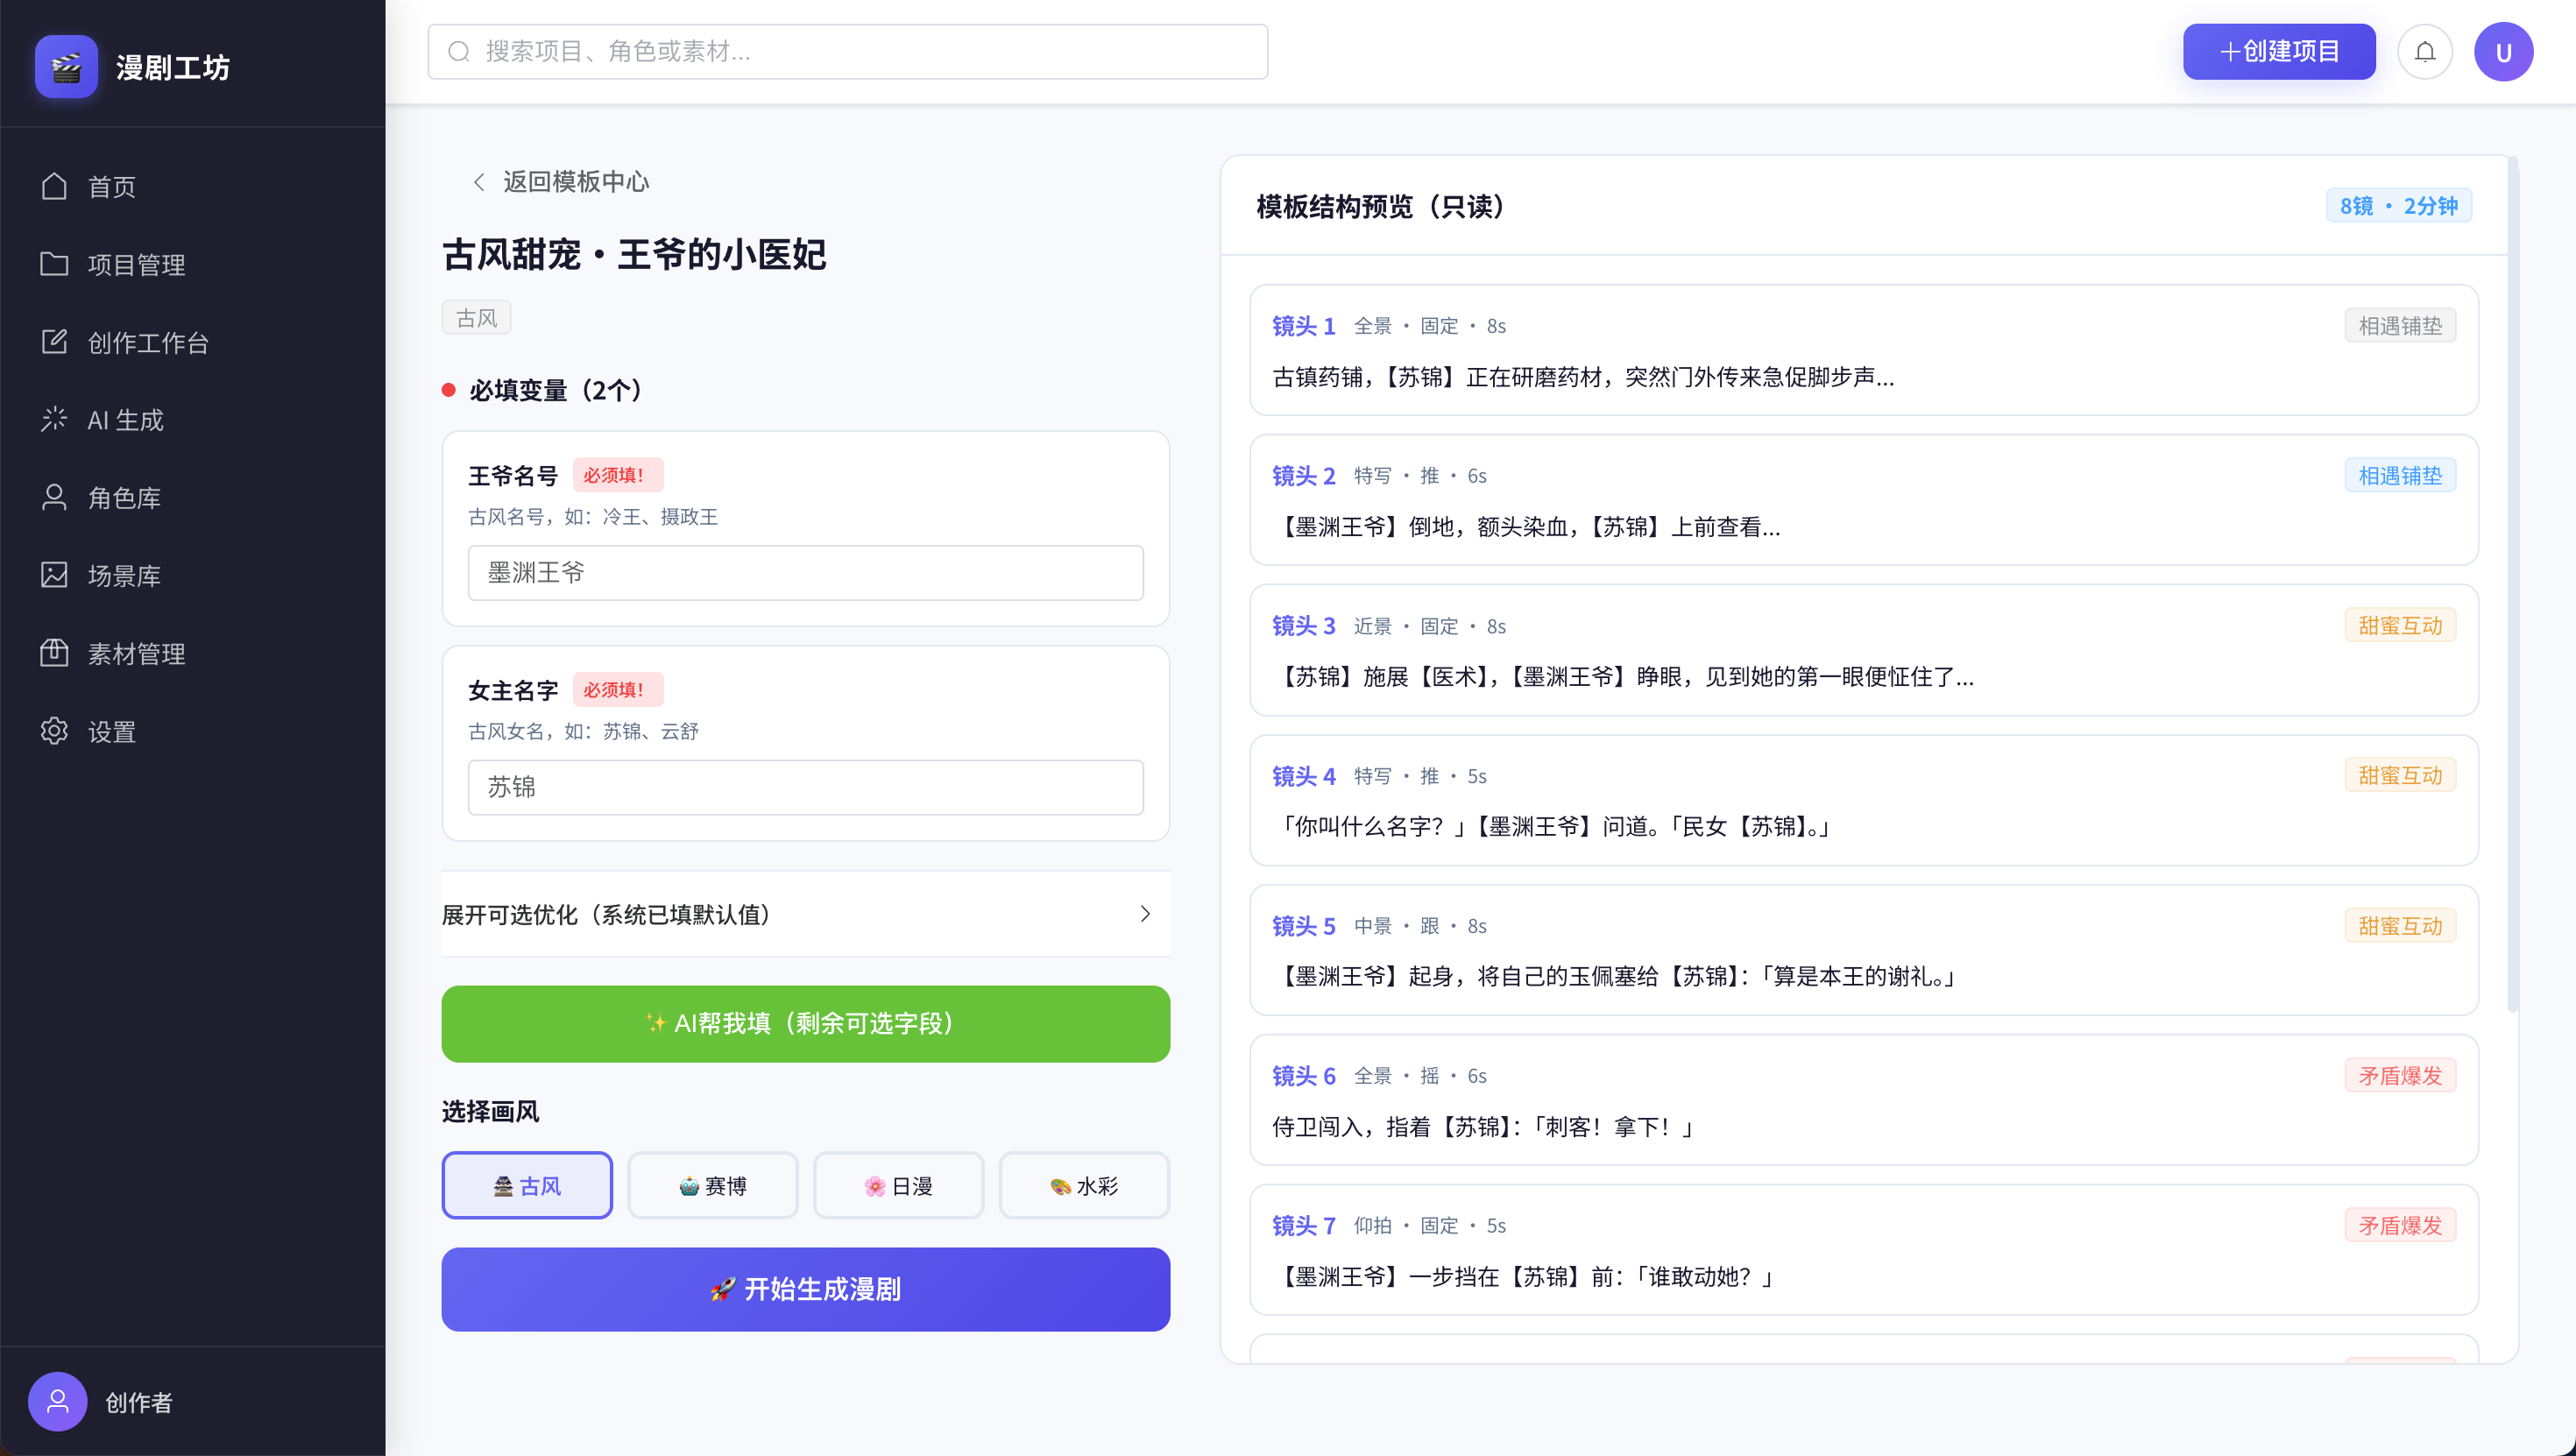
\includegraphics[width=0.88\textwidth]{assets/shot-workspace.png}
\caption{模板工作台（必填变量表单与分镜预览）}\label{fig:shot-workspace}
\end{figure}

\begin{figure}[htbp]
\centering
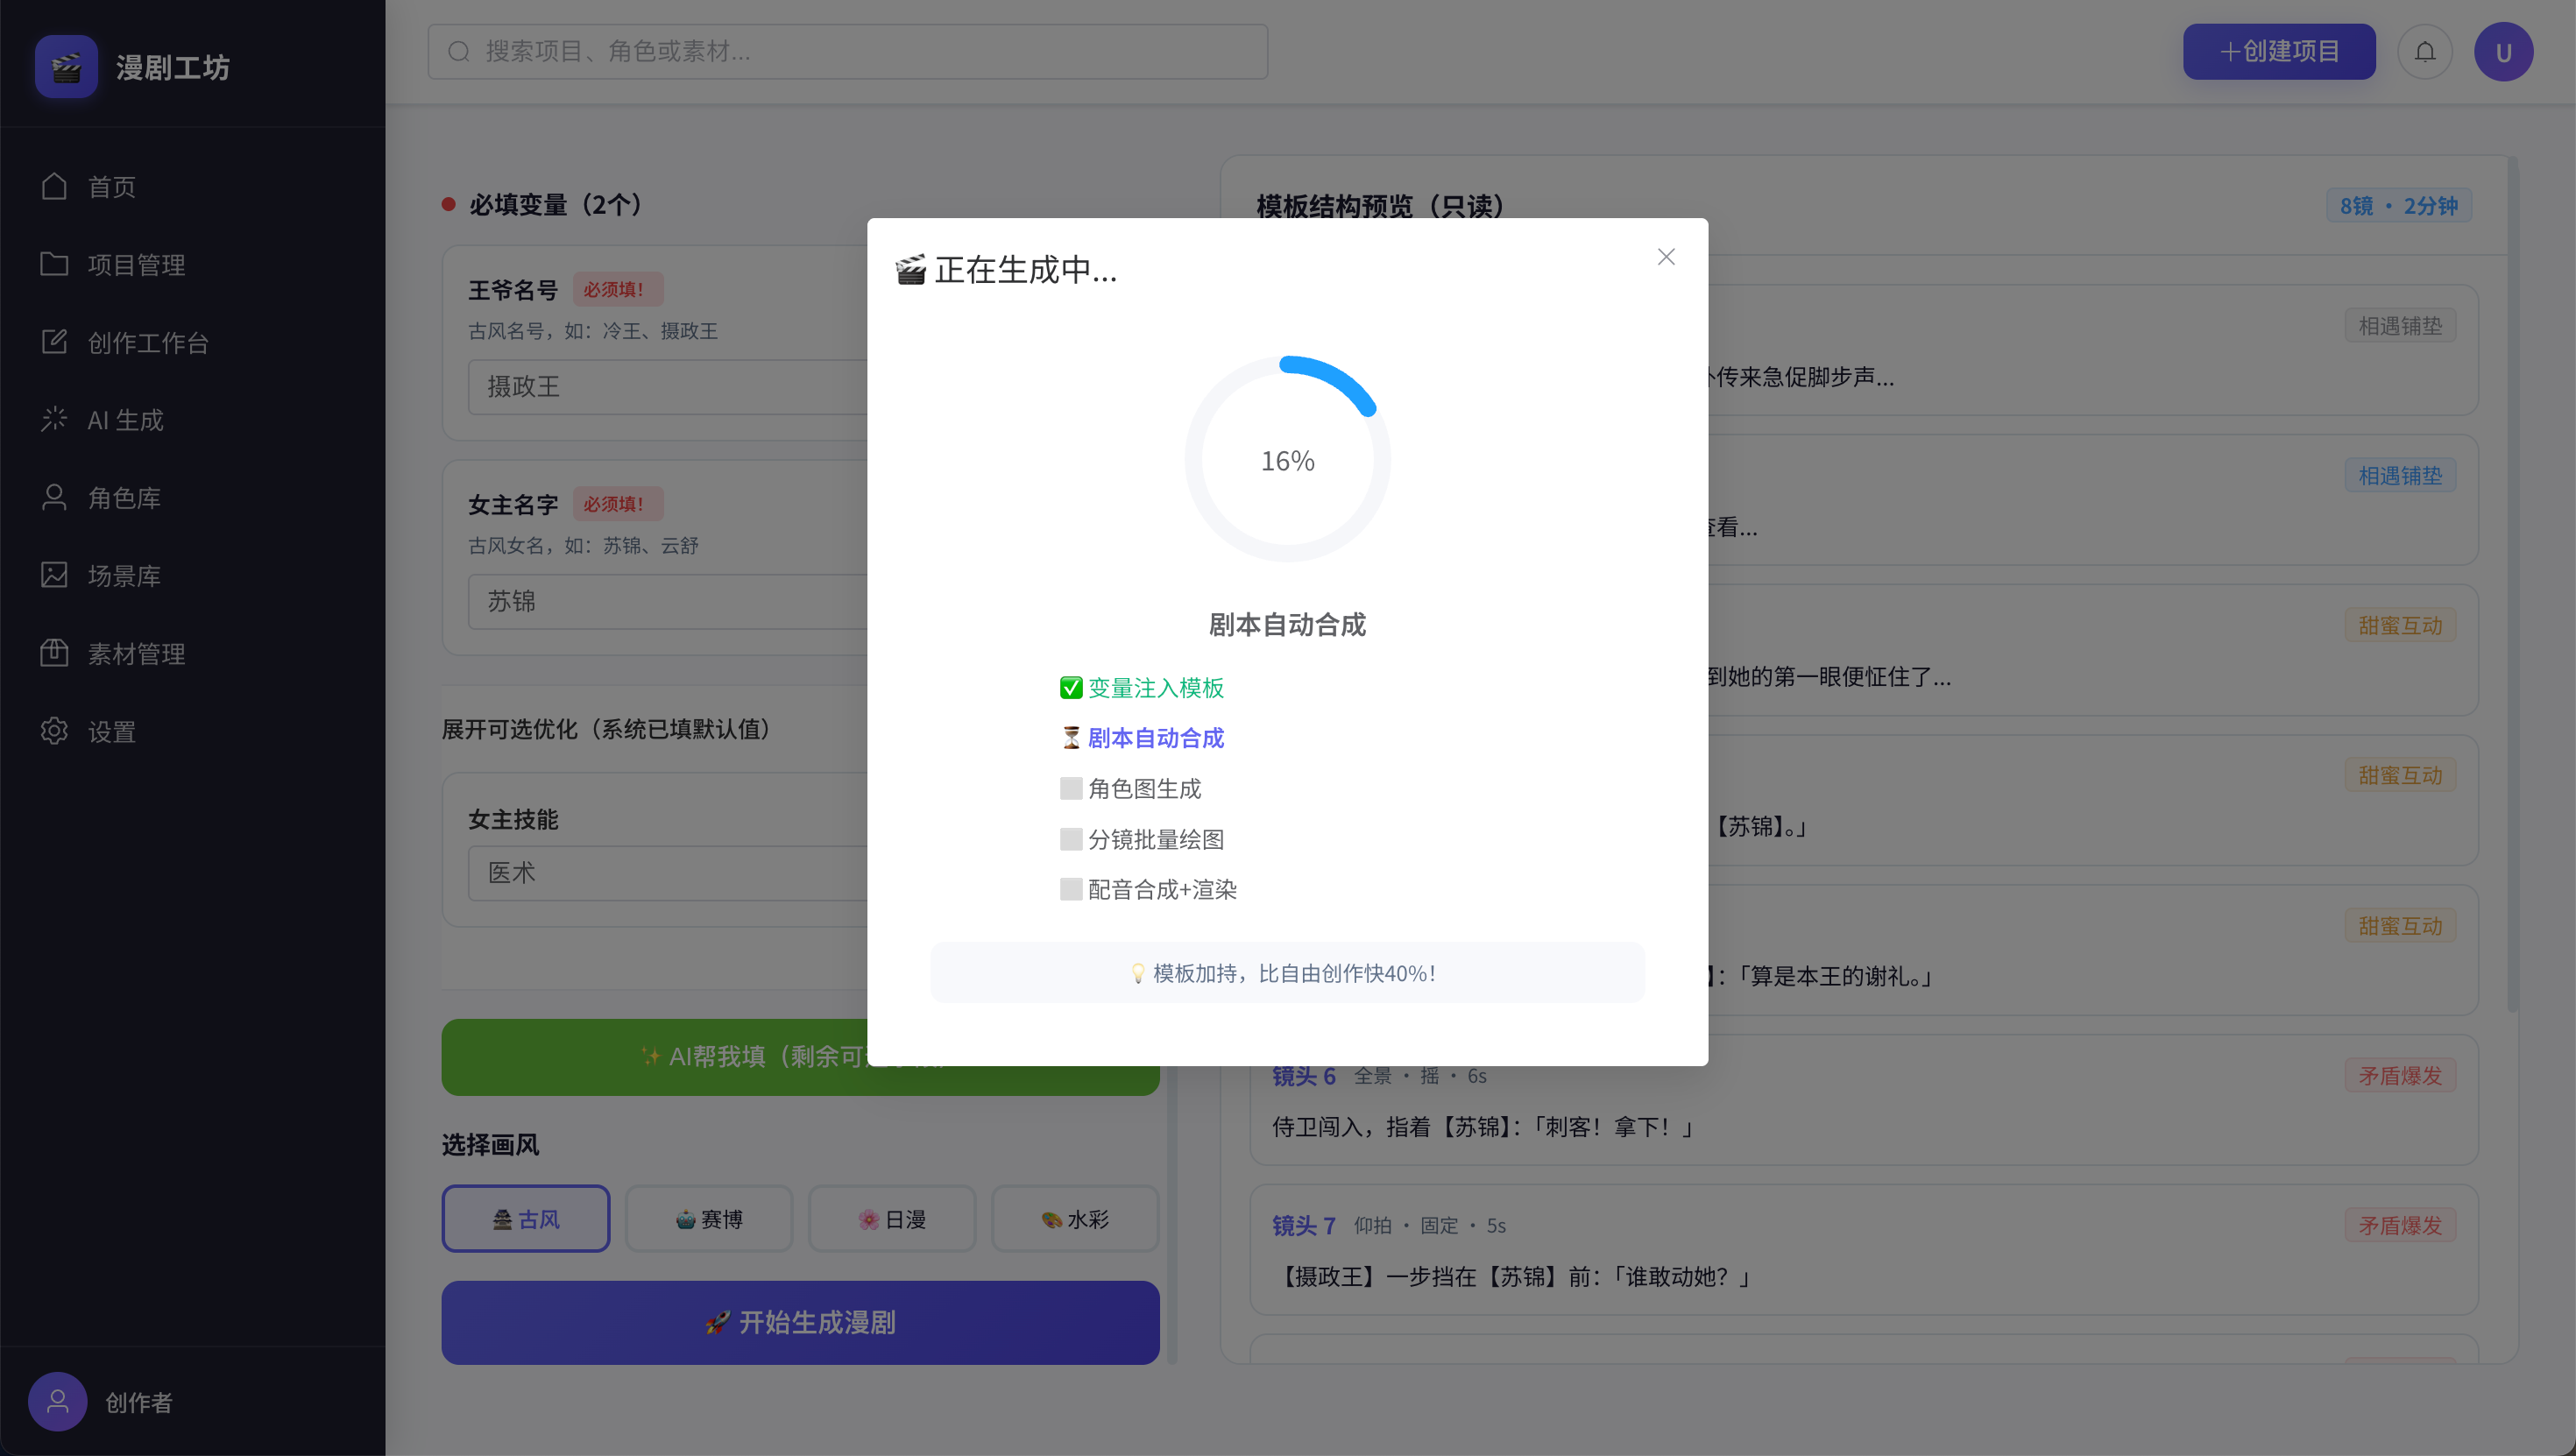
\includegraphics[width=0.88\textwidth]{assets/shot-progress.png}
\caption{生成任务五步进度（状态机实时回传）}\label{fig:shot-progress}
\end{figure}

\begin{figure}[htbp]
\centering
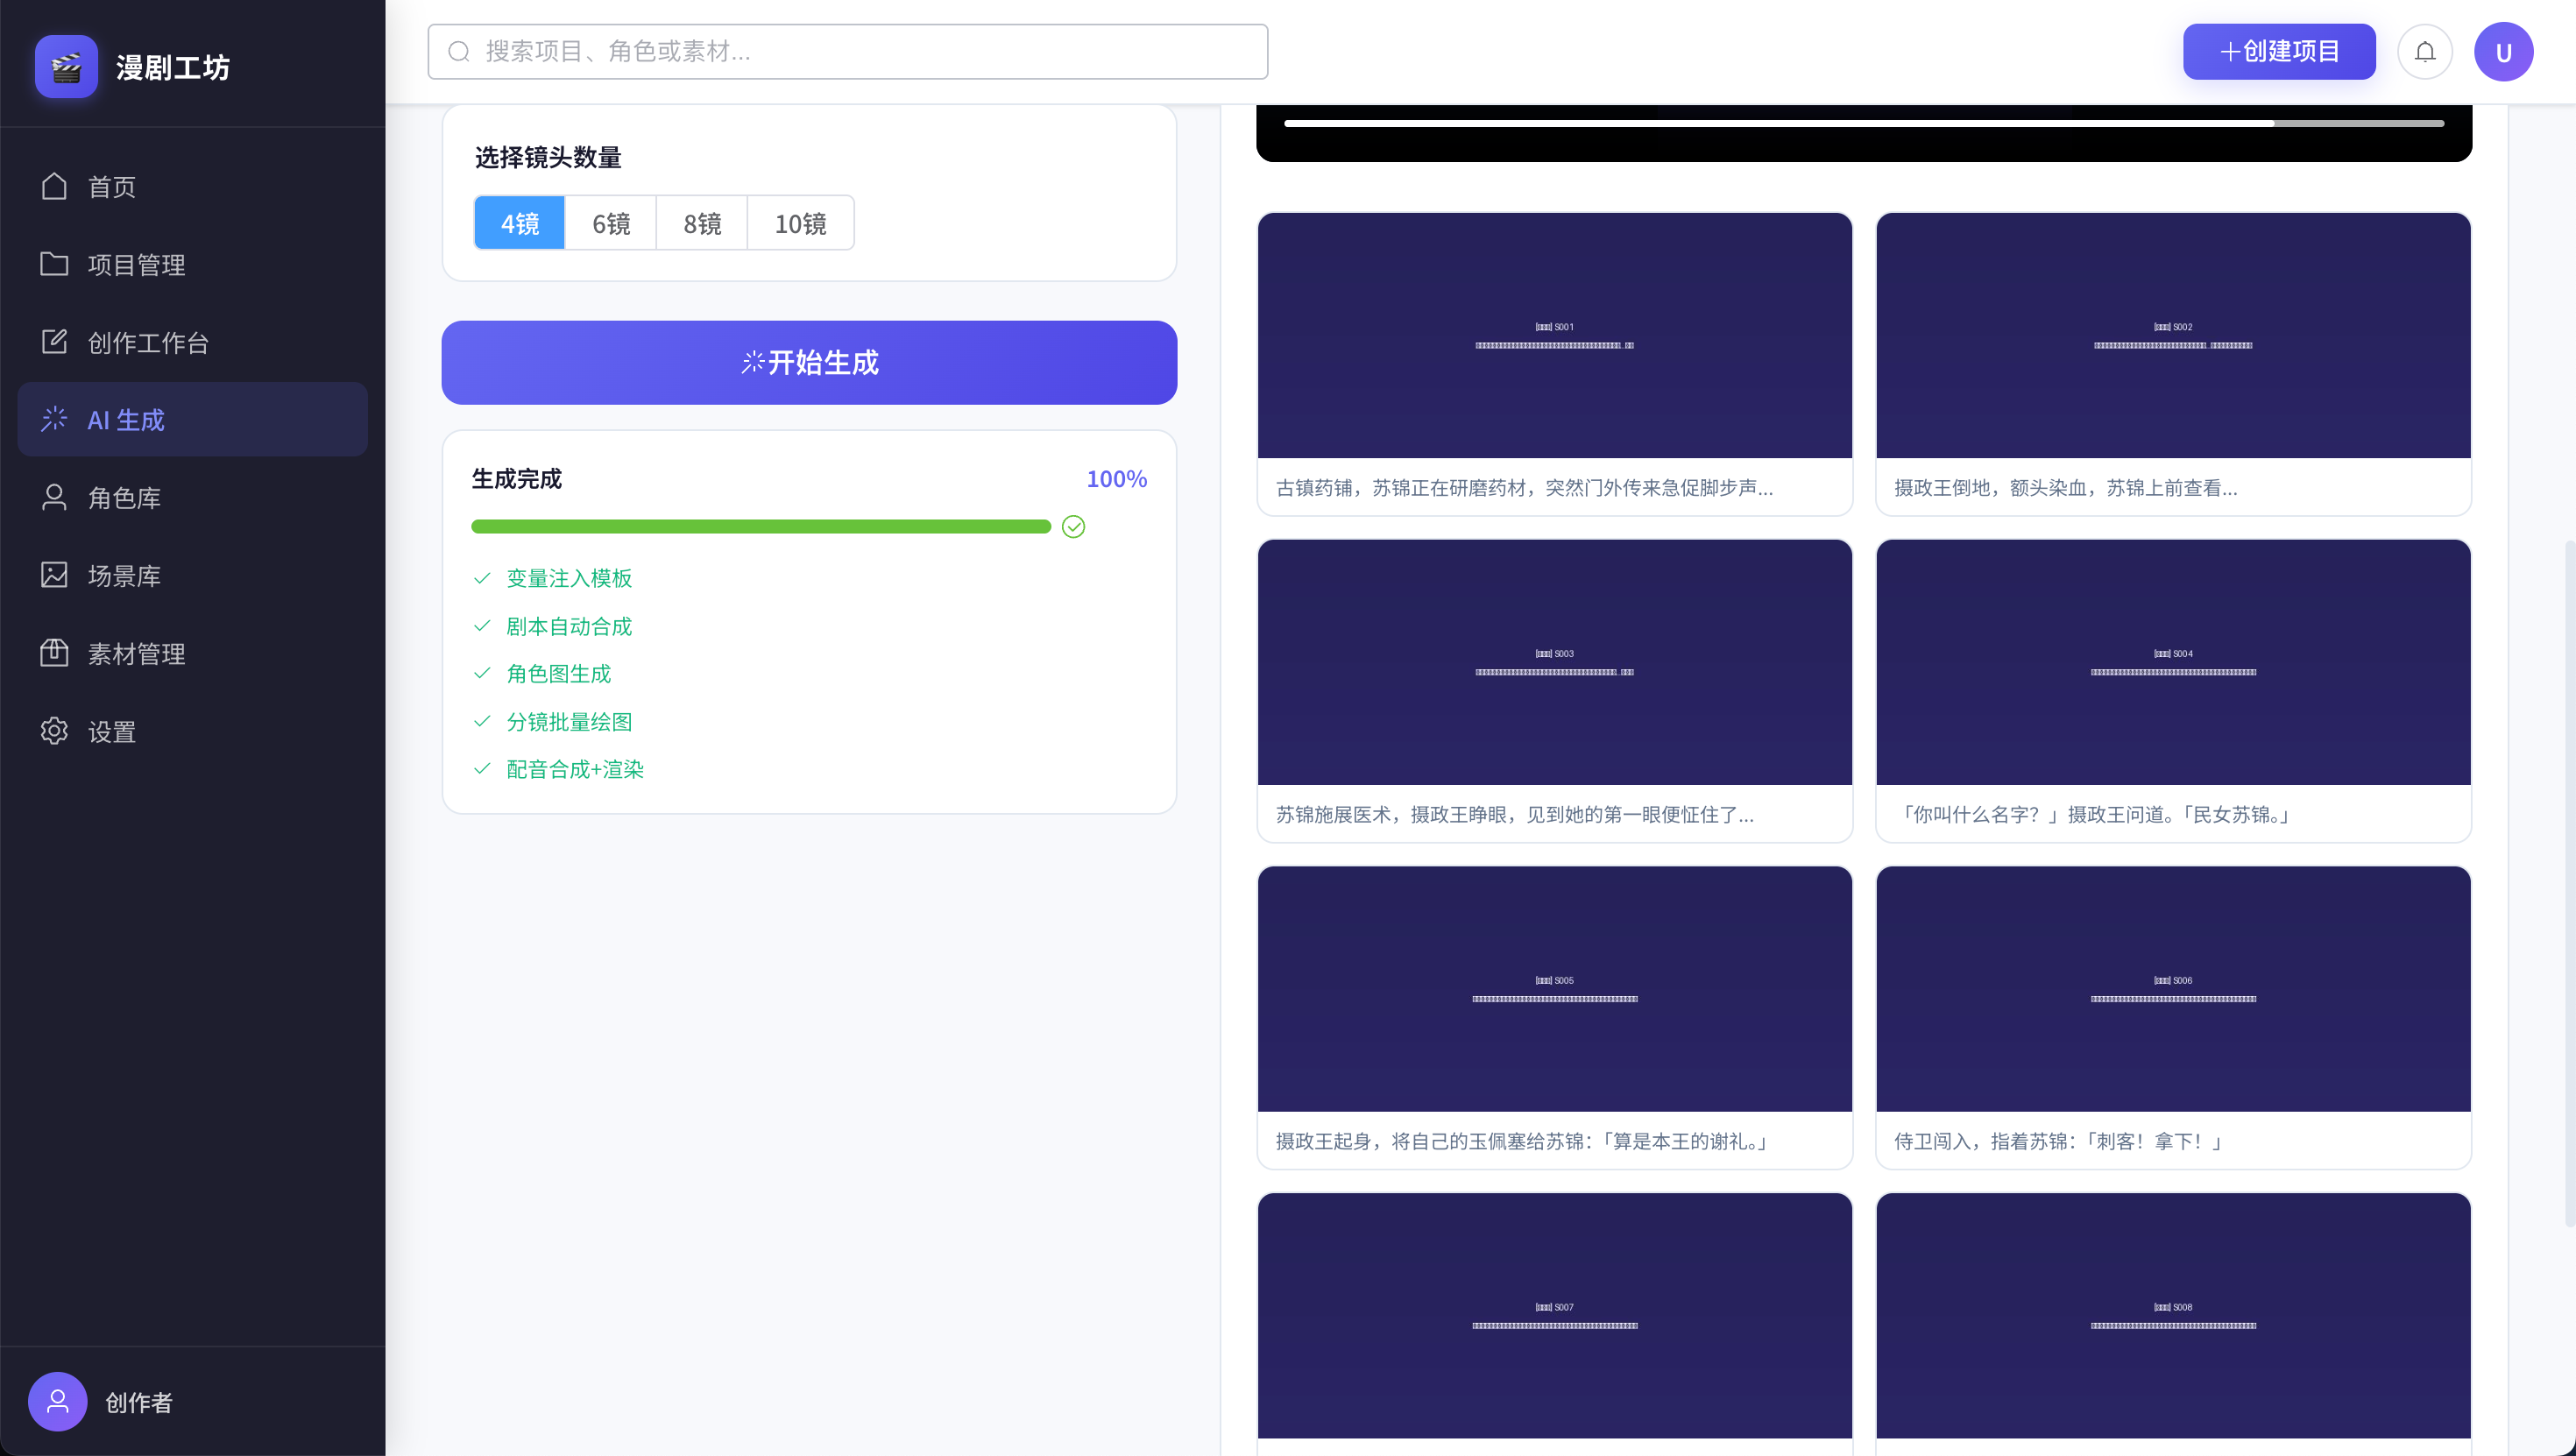
\includegraphics[width=0.88\textwidth]{assets/shot-images.png}
\caption{分镜图片批量生成结果（6 镜并发）}\label{fig:shot-images}
\end{figure}

\begin{figure}[htbp]
\centering
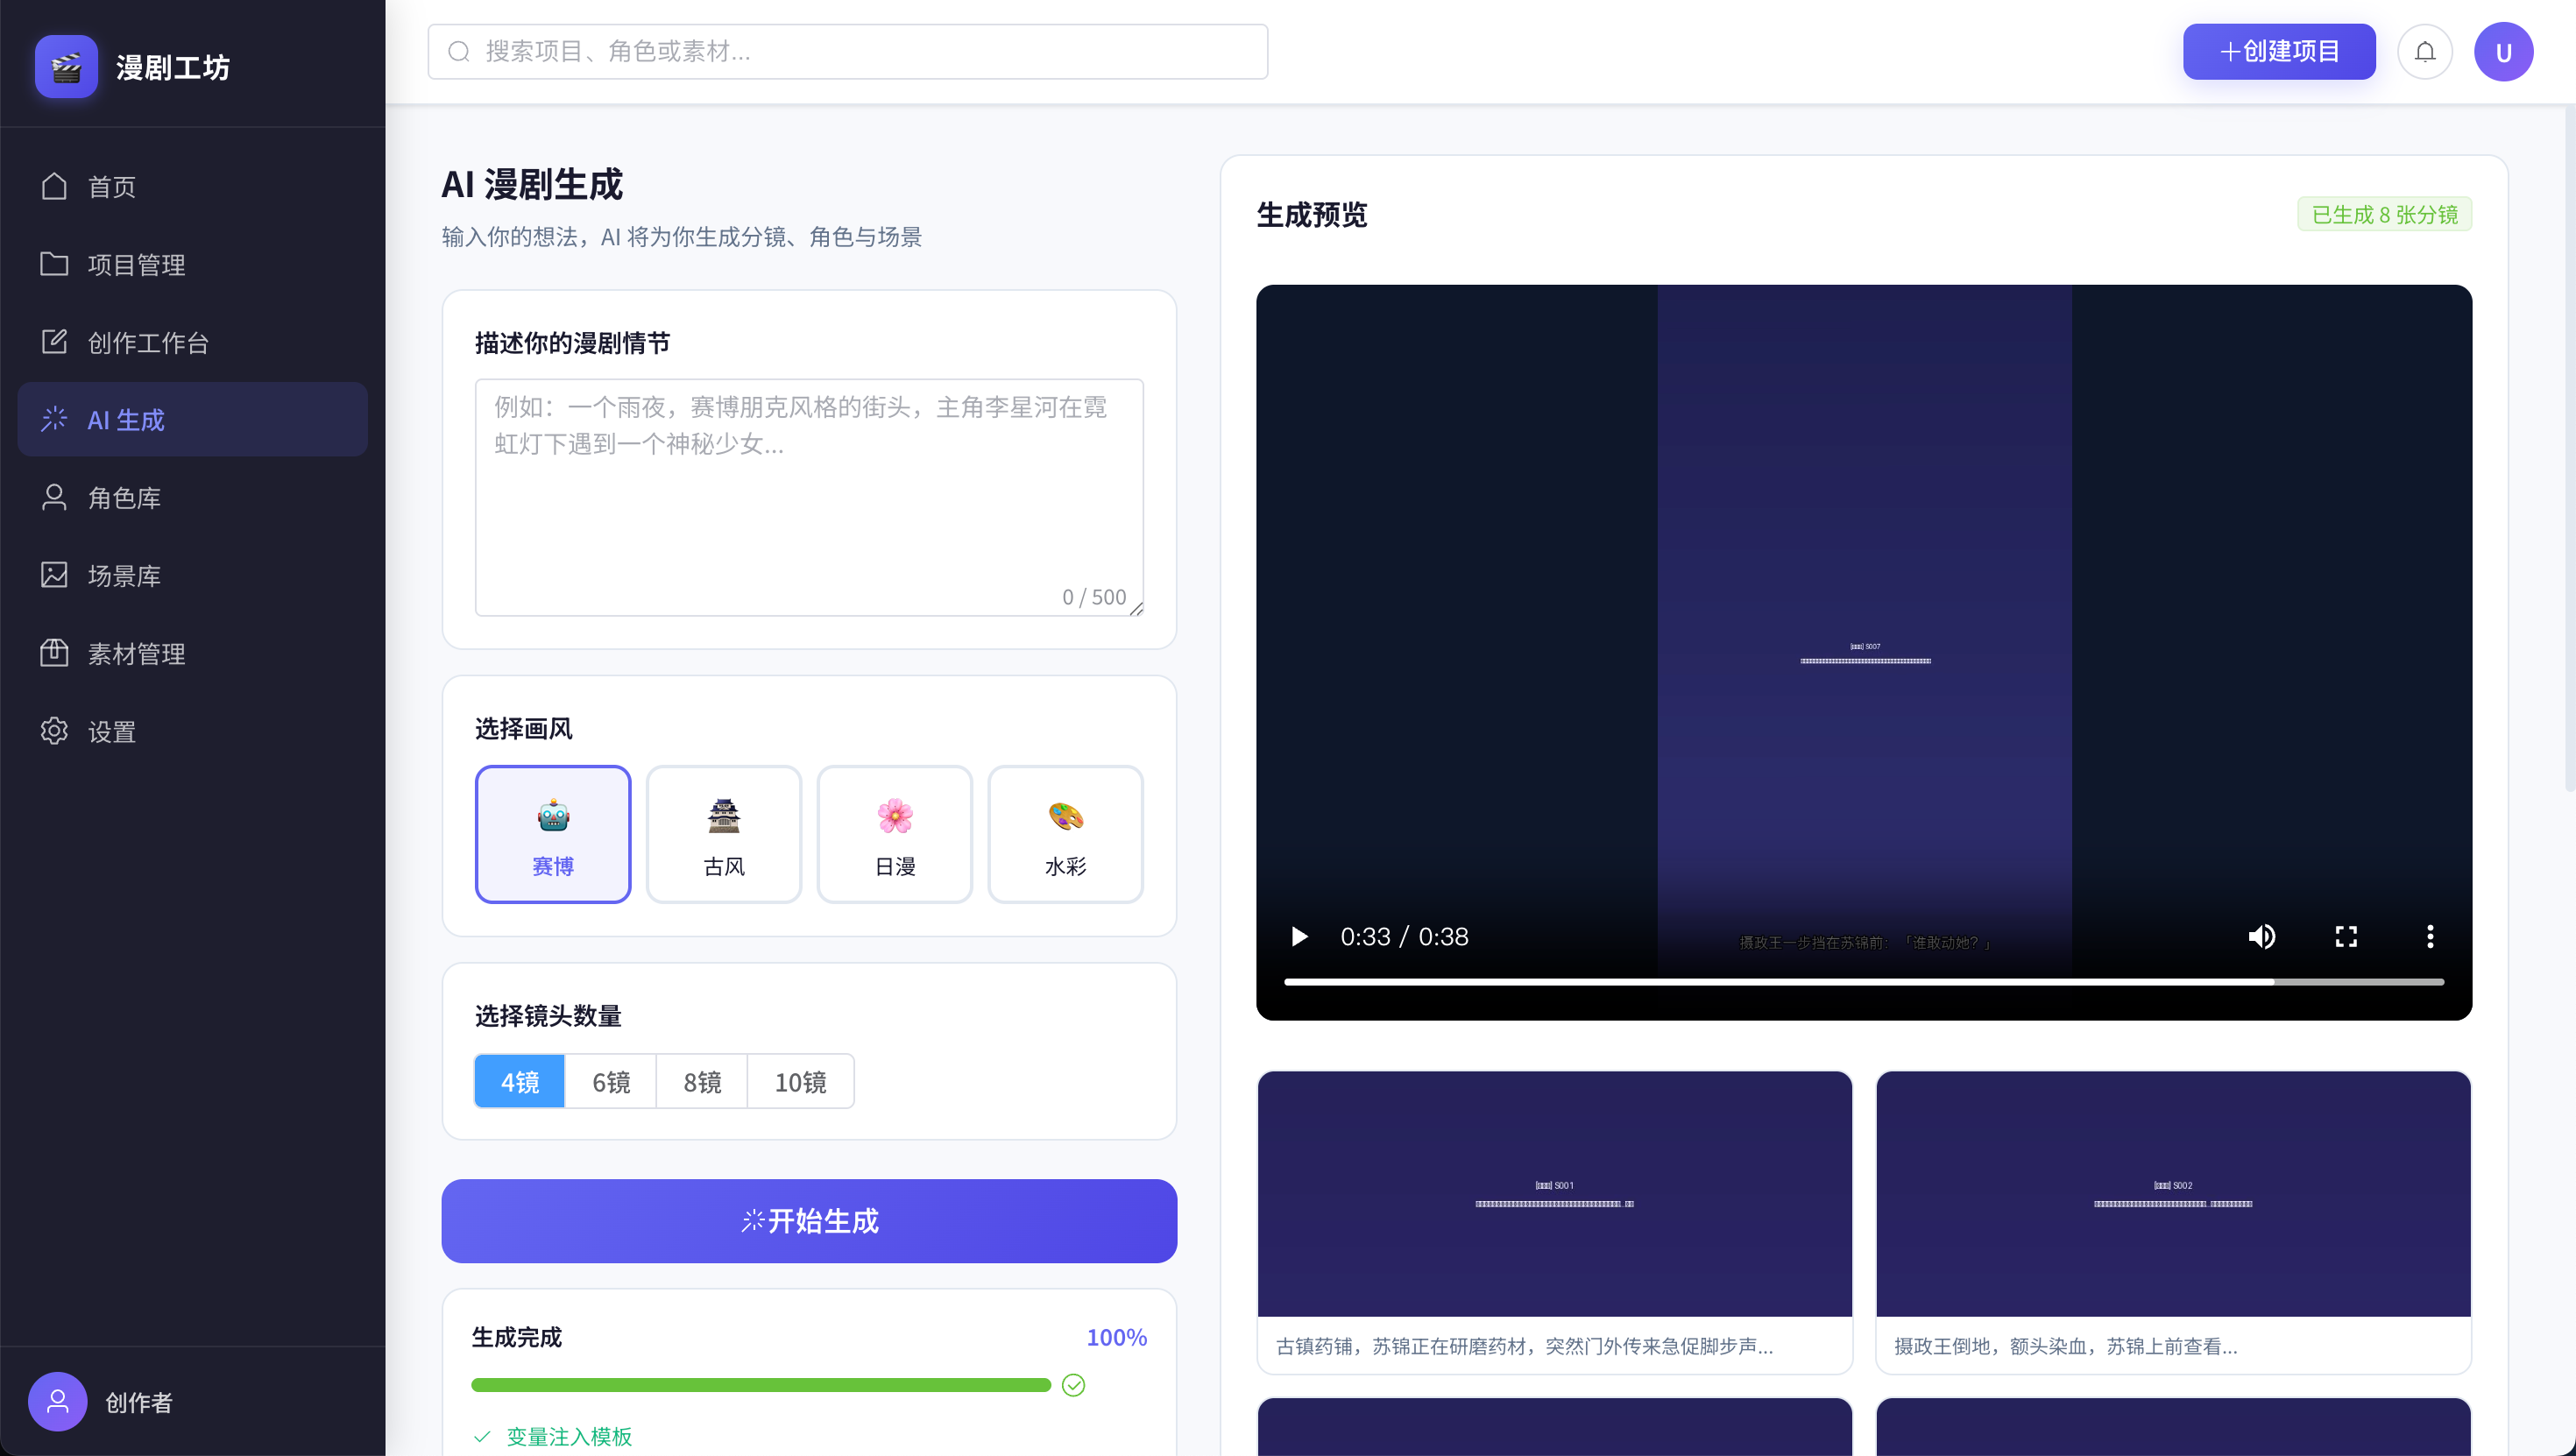
\includegraphics[width=0.88\textwidth]{assets/shot-video.png}
\caption{最终漫剧视频成品（含底部字幕）}\label{fig:shot-video}
\end{figure}

\section{效果展示}

\begin{itemize}
\item \textbf{剧本/分镜}：Mock 分镜接口返回 6 镜结构（镜头类型、机位、台词、情绪），见 \texttt{GET /api/script-generator/mock} 返回 JSON。
\item \textbf{配音}：Mock TTS 按情绪输出不同时长的音频 URL。
\item \textbf{视频成品}：\texttt{/api/video/compose} 合成示例——1080x1920 竖屏、H.264+AAC、时长与音频严格一致、推镜头 + 底部字幕烧录；产物位于 backend/uploads/video\_out/。
\end{itemize}

\section{运行说明}

\begin{lstlisting}[language=bash,caption={项目运行步骤},label=lst:run]
# 1. 后端
cd backend
python3 -m venv venv && ./venv/bin/pip install -r requirements.txt
./venv/bin/python init_db.py          # 初始化数据库与种子数据
./venv/bin/uvicorn app.main:app --reload --port 8000

# 2. 前端
cd frontend
npm install && npm run dev            # http://localhost:5173
\end{lstlisting}

默认账号：\texttt{admin / admin123}（开发模式认证已关闭，登录页保留）。API 文档：\url{http://localhost:8000/api/docs}。

% ============================================================================
\chapter{个人总结与心得}
\section{项目总结}

本项目已完成全部 4 大功能模块与 12 项测试：AI 剧本与分镜生成（M1，含 LLM 调用与 Mock 降级）、分镜图片批量生成（M2，线程池 + 信号量并发调度）、配音合成（M3，情绪驱动时长）、视频合成与剪辑（M4，时长对齐 + Ken Burns + 字幕烧录），并通过模板驱动方案将四模块串联为完整业务闭环。

\textbf{项目亮点}：全流程可在无任何 AI API Key 的本地环境完整演示（Mock 降级设计）；视频合成时长偏差控制在 20ms 量级；模板驱动显著降低使用门槛。

\textbf{项目不足}：真实 AI 引擎（可图/可灵/Edge-TTS）未接入，当前结果为 Mock 数据；视频合成为同步执行，尚不支持任务队列异步化与断点续跑；角色一致性策略（IP-Adapter 方案）为后续规划，尚未实现。

\section{学习收获}

通过本次实训，系统掌握了：LLM 结构化 Prompt 设计与容错解析、多线程并发控制（ThreadPoolExecutor + Semaphore）与任务状态机设计、FFmpeg 滤镜链编程与媒体时长精确控制、Pillow 图像处理与叠加渲染、RESTful 接口设计与前端轮询交互、SQLAlchemy ORM 建模与 JSON 字段应用。对 AIGC 全流程制作的理解也从"各工具拼凑"提升到"平台化编排"层面——真正难的不是单个模型调用，而是\textbf{产物格式统一、流程可观测、环境可降级}的工程化能力。

\section{不足与改进方向}

\begin{enumerate}
\item \textbf{接入真实 AI 引擎}：按抽象接口实现可图（图像）、Edge-TTS（配音）、DeepSeek（已有雏形）的真实实现，替换 Mock。
\item \textbf{任务异步化}：视频合成等耗时操作接入 Celery + Redis 任务队列，支持并发与失败重试。
\item \textbf{角色一致性}：实现 IP-Adapter + 角色参考图方案，结合局部重绘（Inpainting）保证多镜间角色视觉连贯。
\item \textbf{部署上线}：配置前后端构建产物部署与线上环境，接入正式认证鉴权。
\item \textbf{性能优化}：以实测数据对比并发数、编码参数（CRF/预设）对合成耗时与体积的影响，形成优化报告。
\end{enumerate}

\end{document}
